%\documentclass[10pt,a5paper,titlepage,oneside]{book}
%\documentclass{article} % Specifies the document class
%\usepackage[cp1251]{inputenc}

\documentclass[12pt]{article}
\textwidth 150mm
\textheight 240mm
\voffset = -20mm

\usepackage[T1,T2A]{fontenc}
\usepackage[utf8]{inputenc}


%\usepackage[T1,T2A]{fontenc}
%\usepackage[cp1251]{inputenc}


\usepackage[intlimits,sumlimits]{amsmath}

%\usepackage{enumerate,graphicx,dcolumn,amsthm}
\usepackage[russian,ukrainian,english]{babel}
%\usepackage{indentfirst}
%\usepackage{caption}[2013/01/20]
%\captionsetup{labelsep=period,font=sf, labelfont=bf, format=plain, justification=justified, tablename=Таблиця, tablewithin=none}

\usepackage{graphicx}
\graphicspath{{Fig/}}
\usepackage{floatflt}
\usepackage{wrapfig}
\usepackage{afterpage}

\usepackage{tabularx}
\renewcommand{\tabularxcolumn}[1]{m{#1}}
\usepackage{hhline}
\usepackage{multirow}
\usepackage{tabu}

\usepackage{longtable}
\usepackage{colortbl}

\usepackage{tikz}
\usetikzlibrary{calc}
\usepackage{wrapfig}

% \usepackage[left=20mm,right=15mm,top=15mm,bottom=16mm,bindingoffset=0mm,footskip=6mm,includefoot]{geometry}
%\setlength{\parindent}{5mm}
%\usepackage[hang,flushmargin]{footmisc}

%\pagestyle{plain}
%
%
%
%    \usepackage{enumitem}
%    \makeatletter
%        \AddEnumerateCounter{\asbuk}{\@asbuk}{м)}
%    \makeatother
%   \setlist{nolistsep, topsep=0ex, leftmargin=1ex, itemindent=4ex}
%    \renewcommand{\labelenumi}{\arabic{enumi}.}
%    \renewcommand{\labelenumii}{\asbuk{enumii})}




\makeatletter


%\usepackage {titlesec}
%\titleformat{\chapter}{\hyphenpenalty=10000\sf\Large\bfseries}{
%\thechapter. }{0pt}{\Large}
%
%\titlespacing*{\chapter}{0pt}{1.1\baselineskip}{\baselineskip}
%
%\titleformat{\section}{\hyphenpenalty=10000\sf\large\bfseries}{
%\thesection. }{0pt}{\large}
%
%\makeatother




\usepackage{pifont}
% Подключаемый Symbol-шрифт,
% Обеспечивает доступность семейства \verb|U/psy/m/n| под именем greek
\DeclareSymbolFont{greek}{U}{psy}{m}{n}
% Выбор команды переключения шрифта
\DeclareSymbolFontAlphabet{\gr}{greek}



%\renewcommand{\theequation}{\thechapter.\arabic{equation}}

\usepackage{cite}
\bibliographystyle{elsarticle-num}


\begin{document}           % End of preamble and beginning of text.

\begin{center}

{\bfseries Modeling of ideality factor value in $n^+$--$p$--$p^+$--Si structure}

O.Ya. Olikh, O.V. Zavhorodnii

https://orcid.org/0000-0003-0633-5429 (Olikh)

\emph{Taras Shevchenko National University of Kyiv}

\emph{64/13, Volodymyrska Street, City of Kyiv, Ukraine, 01601}

\emph{e-mail: olikh@univ.kiev.ua}

\end{center}

This paper presents the results of computer simulation of the ideality factor of silicon $n^+-p-p^+$ structure with iron contamination.
The Solar Cells Capacitance Simulator (SCAPS) was the tool used for numerical simulation of these devices.
The iron concentration range of $10^{10}-10^{13}$~cm$^{-3}$, acceptor doping level range of $10^{15}-10^{17}$~cm$^{-3}$, temperature range of $290-340$~K,
and base thickness range of $150-240$~$\mu$m were used in the investigation.
The double diode model was used to extract the ideality factor.
The following cases were considered: 
(i)~uniformly distributed lone interstitial iron atoms;
(ii)~coexistence of non--uniformly distributed $\mathrm{Fe}_i$ and $\mathrm{Fe}_i\mathrm{B}_s$
It has been shown that 
the ideality factor value determined by a hole occurring on the $\mathrm{Fe}_i$ level, 
a trap location, and a intrinsic recombination contribution.
The increase in base thickness leads to decrease in $n$ value.
The sign of change in ideality factor after $\mathrm{Fe}_i\mathrm{B}_s$ dissociation depends on temperature, doping level, and iron concentration.


\textbf{Key words:}
ideality factor, silicon, $n^+$--$p$--$p^+$ structure, SCAPS, iron concentration


\section{Introduction}

In the literature, there are several models that describe the current--voltage ($I-V$) characteristics of the solar cells (SCs).
These models contain some parameters, which reflect the processes within the structures and are related to the main characteristics of the photovoltaic conversion.
So single diode model with three parameters has been used to represent the SC static characteristic because of simplicity:
\begin{equation}
\label{eqIVs}
    I=I_{0}\left[\exp\left(-\frac{qV}{nkT}\right)-1\right]-I_{ph}\,,
\end{equation}
were
$I_0$ is the saturation current,
$n$ is the diode ideality factor,
$I_{ph}$ is the total current generated by solar cell.
The ideality factor value indicates about a defect related recombination and directly determines open--circuit magnitude:
\begin{equation}
\label{eqVoc}
    V_{oc}=\frac{nkT}{q}\ln\left(\frac{I_{ph}}{I_0}+1\right)\,.
\end{equation}
Eq.~(\ref{eqIVs}) does not take into account a leakage current, a series losses of load current.
Besides, the widely used double diode model is developed by considering the effect of recombination current loss
in the depletion region \cite{2Diod:Ishaque,2Diod:Buhler,Breitenstein2013}:
\begin{equation}
\label{eqIVd}
    I=I_{01}\left[\exp\left(-\frac{q(V-R_sI)}{kT}\right)-1\right]
      + I_{02}\left[\exp\left(-\frac{q(V-R_sI)}{nkT}\right)-1\right]
      +\frac{V-R_sI}{R_{sh}}
      -I_{ph}\,,
\end{equation}
where
first term closely related to the recombination in the quasi--neutral region,
second term describes the overall space charge region (SCR) recombination,
$R_s$ and $R_sh$ are the series and shunt resistance, respectively.
In this case the relationship between the ideality factor and SC characteristics is more complicated.
Певні приклади щодо взаємозв'язку n з напругою холостого ходу та fill factor  рамках дво-діодної моделі можна знайти в \cite{Olikh2018SM}.
Typically, the value of the ideality factor ranges from 1 to 2 for real devices and depends on ambient conditions and recombination center parameters,
including the concentration of traps \cite{n2_Beier,n2McIntosh,n2Kaminski,HAMEIRI2013251,Heide}.
This makes the ideality factor an important parameter that can be used to describe the electrical behavior of photovoltaic devices and characterize the recombination in SCs \cite{Duan}.

One of the main obstacles of such a convenient and express method developing is the multiparameter relationship between
the $n$ value and the concentration of recombination centers.
This paper attempts to get over these difficulties by the simulation of $I-V$ characteristic of silicon solar cells,
the determination of ideality factor, and the study of  $n$ value depending on simulation parameters.
In contrast to the previous paper \cite{Olikh2019SM} in this case the $n^+$--$p$--$p^+$-structure,
which is closer to the real SC, is under consideration.
Additionally the base thickness is known \cite{Sach_d,FeB:Schmidt} to affect SC efficiency;
therefore the paper considers the influence of this parameter on the ideality factor value.

The paper focuses on the case when the main recombination centers are the iron related defects.
On the one hand, the iron atoms  are one of the most common as well as the most harmful impurities in silicon solar cell.
On the other hand, the $\mathrm{Fe}_i\mathrm{B}_s$ pairs can be readily dissociated by illumination \cite{FeB:Schmidt};
the association reaction can take place when exposed in darkness for ten minutes \cite{FeB:kinetic}.
Such a change in recombination center state should lead to a change in a ideality factor value,
that is easy to obtain experimentally and to use to SC characterization.
Therefore, the paper also pays attention to dependencies of $n$ value change.

\section{Simulation details}

The calculation presented here uses $n^+-p-p^+$ structure shown in inset in Fig.~\ref{FigIV}.
Its main parts are the emitter layer with thickness $d_n$, the base with hole conductivity and thickness $d_p$
and the $p^+$ layer with thickness $d_{BSF}$ intended to back surface field (BSF) creation.
BSF-layer is designed to increase the photovoltaic converter efficiency by reducing the losses concerned with surface recombination
and such structure is widely used for both manufacturing of real solar cells and modeling \cite{SCAPSuseSi4,SCAPSuseSi1,SCAPSuseSi5}.

The material of all layers was assumed to be monocrystalline silicon.
The temperature dependencies of bandgap was calculated according to P\"assler equations \cite{Pasler}.
The bandgap narrowing, thermal carrier velocities,
and  free carrier effective mass
were taken from Yan and Cuevas \cite{EgNarrow}, Green \cite{Nc:Green}, and O'Mara \emph{et al.} \cite{OMara}, respectively.
Data from Couderc~\emph{et al.} \cite{Si_ni_Couderc} were used to evaluate intrinsic carrier density and density of states effective masses.
The temperature dependencies carrier mobilities were described by Klaassen's theory \cite{KLAASSEN953,Hull}.

It was assumed uniform doping with phosphorus (the emitter layer, concentration $N_\mathrm{D}$)
and boron (base and BSF--layer, concentrations $N_\mathrm{A}$ and $N_\mathrm{BSF}$, respectively).

The following recombination processes were taken into account:
i)~the outside surface recombination with electron and hole velocities $10^3$~cm/s;
ii)~the intrinsic recombination (radiative band--to--band and Auger with coefficients,
which depend on temperature and doping level according
to Nguyen~\emph{et al.} \cite{Si_BtB} and Altermatt~\emph{et al.} \cite{Si_Auger});
iii)~the Shockley–-Read-–Hall (SRH) recombination.

In the last case, as the base and BSF--layer uniform contaminant, iron is assumed to be in concentration $N_\mathrm{Fe}$.
It is well known that the iron atom locates in lone interstitial lattice position in silicon ($\mathrm{Fe}_i$) or
interacts with ionized acceptors and combines into $\mathrm{Fe}_i\mathrm{B}_s$ pair.
The two cases were under consideration.
In the first one, uniformly distributed $\mathrm{Fe}_i$ with concentration $N_\mathrm{Fe}$ was assumed.
Such case is realizing under constant illumination or immediately after its termination.
The temperature independent donor level $E_{\mathrm{Fe}_i} = E_V+0.394$~eV \cite{Rein2,MurphyJAP2011,Kohno}
and electron $\sigma_{n,{\mathrm{Fe}}}=3.47\times10^{-15}T^{-1.48}$~m$^2$ and
hole $\sigma_{p,{\mathrm{Fe}}}=4.54\times10^{-20}\exp\left(-\frac{0.05}{kT}\right)$~m$^2$ capture cross-sections \cite{ROUGIEUX2018,Paudyal}
are associated with $\mathrm{Fe}_i$.
In the second one, $\mathrm{Fe}_i$ and $\mathrm{Fe}_i\mathrm{B}_s$ were coexistence.
Their concentration were non--uniformly distributed through base and BSF--layer.
The more details are presented elsewhere \cite{Olikh2019SM} and the representative
examples of calculation are shown in Fig.~\ref{FigEf}.
Such case is realizing under dark equilibrium condition.
The $\mathrm{Fe}_i\mathrm{B}_s$ is amphoteric defect and donor level $E_{\mathrm{FeB}}^\mathrm{D}= E_V+0.10$~eV,
$\sigma_{n,{\mathrm{FeB}}}^\mathrm{D}=4\times10^{-17}$~m$^2$,
$\sigma_{p,{\mathrm{FeB}}}^\mathrm{D}=2\times10^{-18}$~m$^2$
and acceptor level $E_{\mathrm{FeB}}^\mathrm{A}= E_C-0.26$~eV,
$\sigma_{n,{\mathrm{FeB}}}^\mathrm{A}=5.1\times10^{-13}T^{-2.5}$~m$^2$,
$\sigma_{p,{\mathrm{FeB}}}^\mathrm{A}=3.32\times10^{-14}\exp\left(-\frac{0.262}{kT}\right)$~m$^2$
\cite{Istratov1999,Rein2,MurphyJAP2011,ROUGIEUX2018,Paudyal,Wijaranakula}
are used in simulation.

The dark forward dark $I-V$ characteristic were generated by
one-dimensional code SCAPS~3.3.08 \cite{SCAPS1,SCAPS2}
over a voltage range up to $0.45$~V with step 0.01~V.
This software is widely applied in modeling various solar cells \cite{SCAPSuse1,SCAPSuse2,SCAPSuse3,SCAPSuse5,SCAPSuseSi1,SCAPSuseSi4,SCAPSuseSi3},
silicon based devices including \cite{SCAPSuseSi1,SCAPSuseSi3,SCAPSuseSi4}.
The used parameters are listed in Table~\ref{tabParametr}.
Thus, the varied parameters were the boron concentrations in the base, iron concentration, base thickness and temperature.
Taking into account two defect configuration, 15048 structures were simulated.
The examples of $I-V$ curve are shown in Fig.~\ref{FigIV}.

The simulated $I-V$ characteristic were fitted by following equation:
\begin{equation}
\label{eqIV}
    I=I_{01}\left[\exp\left(-\frac{qV}{kT}\right)-1\right]+ I_{02}\left[\exp\left(-\frac{qV}{nkT}\right)-1\right]\,.
\end{equation}
Eq.~(\ref{eqIV}) corresponds to the dark double diode model with neglected both series and shunt resistances.
The first diode represents the ``ideal'' diode, describing the so--called diffusion current characterized by a saturation current $I_{01}$,
and the second diode is the so--called recombination current, characterized by the saturation current $I_{02}$ and ideality factor $n$ \cite{Breitenstein2013}.
$n$, $I_{01}$, and $I_{02}$ were taken as fitting parameters and the meta--heuristic method IJAVA \cite{IJAVA} was used.
The representative results of the fitting are shown in Fig.~\ref{FigIV} as well.


In the case of lone unpaired $\mathrm{Fe}_i$ the following value were calculated:
$n_\mathrm{Fe}^\mathrm{srh}$ is the ideality factor if the SRH recombination was taken into account only;
$n_\mathrm{Fe}$ is the ideality factor if the both SRH recombination and intrinsic recombination were allowed;
$\delta n_\mathrm{Fe}^\mathrm{srh}=n_\mathrm{Fe}^\mathrm{srh}-n_\mathrm{Fe}$ characterizes the influence of intrinsic recombination on ideality factor value.
In the case of $\mathrm{Fe}_i\mathrm{B}_s$ and $\mathrm{Fe}_i$ coexistence the
$n_\mathrm{FeB}^\mathrm{srh}$, $n_\mathrm{FeB}$, $\delta n_\mathrm{FeB}^\mathrm{srh}=n_\mathrm{FeB}^\mathrm{srh}-n_\mathrm{FeB}$ were calculated (indices had the same meaning).
Besides, the change of the ideality factor after $\mathrm{Fe}_i\mathrm{B}_s$ association $\delta n_\mathrm{Fe-FeB}=n_\mathrm{Fe}-n_\mathrm{FeB}$ was calculated as well.






%In the case of unpaired $\mathrm{Fe}_i$ sole (under constant illumination or immediately after its termination) the following value were calculated:
%$n_\mathrm{Fe}^\mathrm{srh}$ is the ideality factor if the SRH recombination was taken into account only;
%$n_\mathrm{Fe}$ is the ideality factor if the both SRH recombination and intrinsic recombination were allowed;
%$\delta n_\mathrm{Fe}^\mathrm{srh}=n_\mathrm{Fe}^\mathrm{srh}-n_\mathrm{Fe}$ characterizes the influence of intrinsic recombination on ideality factor value.
%In the case of $\mathrm{Fe}_i\mathrm{B}_s$ and $\mathrm{Fe}_i$ coexistence (dark equilibrium condition) the
%$n_\mathrm{FeB}^\mathrm{srh}$, $n_\mathrm{FeB}$, $\delta n_\mathrm{FeB}^\mathrm{srh}=n_\mathrm{FeB}^\mathrm{srh}-n_\mathrm{FeB}$ were calculated (indices had the same meaning).
%Besides, the change of the ideality factor after $\mathrm{Fe}_i\mathrm{B}_s$ association $\delta n_\mathrm{Fe-FeB}=n_\mathrm{Fe}-n_\mathrm{FeB}$ was calculated as well.



% \begin{equation}
%\label{eqNFeB}
%    N_{\mathrm{FeB}}=N_{\mathrm{Fe}}\frac{N_\mathrm{A}10^{-23}\exp\left(-\frac{E_b}{kT}\right)}
%     {\left[1+N_\mathrm{A}10^{-23}\exp\left(-\frac{E_b}{kT}\right)\right]\left[1+\exp\left(-\frac{F-E_{\mathrm{Fe}_i}}{kT}\right)\right]}\,.
%\end{equation}


\section{Results and discussion}

Типові отримані в результаті симулювання залежності величини фактору неідеальноті від температури та концентрацій бору та заліза представлені на рисунках~\ref{FigTNa},\ref{FigTNfe}, \ref{FigNaNfe}.
Зауважим, що на тих рисунках, де поверхня для $\delta n_\mathrm{Fe}^\mathrm{srh}$ (number 5, orange) не показана, вона практично збігається з к поверхнею для $\delta n_\mathrm{FeB}^\mathrm{srh}$ (number 4, yellow).

Декілька важливих висновків, необхідних для аналізу отриманих даних, можно зробити з рис.\ref{FigEf}.
Перед безпосереднім аналізом отриманих залежностей необхідно звернути увагу на рис.\ref{FigEf}.
По-перше, він свідчить, що навіть для випадку, коли переважаюча частина
атомів заліза утворила пари з  акцепторною домішкою,
In the case of $\mathrm{Fe}_i\mathrm{B}_s$ and $\mathrm{Fe}_i$ coexistence
рекомбінаційні процеси визначаються насамперед, неспареними міжвузольними дефектами.
In fact, донорний рівень $E_{\mathrm{FeB}}^\mathrm{A}$ знаходить нижче рівня Фермі і тому ймовірність захоплення ним нерівноважних електронів достатньо мала.
Крім того, у 2/3 глибини ОПЗ, з процесами у якому насамперед пов'язують появу фактор неідеальності,
кількість неспарених атомів заліза переважає кількість пар.
Це підтверджується і тим, що залежності $n_\mathrm{FeB}$ (surfaces 1, red) and $n_\mathrm{Fe}$ (surfaces 2, cyan) on Figs.~\ref{FigTNa}--\ref{FigNaNfe} мають однаковий характер.
По-друге, кількість неспарених атомів заліза In the case of $\mathrm{Fe}_i\mathrm{B}_s$ and $\mathrm{Fe}_i$ coexistence може бути досить значною і зростає зі збільшенням температури та
зниженням ступеня легування.
Так, наприклад, при $T=340$~K and $N_\mathrm{A}=10^{15}$~cm$^{-3}$ (or $10^{16}$~cm$^{-3}$) у квазінейтральній області бази
концентрація $\mathrm{Fe}_i$  досягає 23 (or 3) відсотків $N_\mathrm{Fe}$.
Тобто в цих умовах, концентрація неспарених атомів заліза в темряві при $N_\mathrm{Fe}=10^{13}$~cm$^{-3}$ більша
ніж при освітленні та $N_\mathrm{Fe}=10^{11}$~cm$^{-3}$.
Нарешті, так як лише $\mathrm{Fe}_i^+$ на відміну від $\mathrm{Fe}_i^0$ беруть участь у рекомбінації ІКР,
то ці процеси ефективно відбуваються при $x\geq0.6W_p$ (where $W_p$ - ширина область).
Тобто, при збільшенны рівня легування область, де відбуваються процеси, що визначають величину фактору неідеальності віддаляється від $p-n$ переходу.


При аналізі залежностей фактору неідельності від температури та концентрації бору необхідно враховувати декілька факторів. А саме.

i)~The recombination efficiency is determined by a hole occurring on the $\mathrm{Fe}_i$ level.
Відповідно до статистики Фермі-Дірака у не виродженому напівпровіднику p-типу за умови повної іонізації акцепторів, ймовірність
The probability of hole occupation is

\begin{equation}
\label{eqfp}
 f_p=\frac{1}{1+\frac{N_V(T)}{N_\mathrm{A}}\exp\left(\frac{E_V-E_{\mathrm{Fe}_i}}{kT}\right)}\,.
\end{equation}

Як показано раніше  \cite{Olikh2018SM}, залежність $f_p(T,N_\mathrm{A})$ загалом подібна до тієї, що спостерігається для фактору неідеальності.
Зокрема, коли  $f_p$ близька до одиниці (високі значення $N_\mathrm{A}$ та низькі температури) ця функція змінюється повільно, $n$ практично не залежить від температури і повільно зростає зі збільшенням рівня легування --- Figs.\ref{FigTNfe}(b),(c); \ref{FigNaNfe}(a).
При зменщенні $N_\mathrm{A}$ or (and) increase in T у досить вузькому інтервалі аргументів рівень заповнюється електроном, SRH рекомбінація перестає відбуватися, значення факторунеідеальності  різко падає - Figs.\ref{FigTNa}, \ref{FigTNfe}(a); \ref{FigNaNfe}(b).

ii)~Співвідношення рекомбінації на дефектах та власної.
Загалом наявність SRH рекомбінації викликає зростання $n$, у граничному випадку
If the defect related recombination is dominant, the value often reported in publications is $n=2$.
radiative band--to--band and Auger інтенсифікується при збільшенні концентрації вільних носіїв заряду (рівня легування) та температури \cite{Si_BtB,Si_Auger}).
При цьому
о фактор неідеальності падає, а величини
$\delta n_\mathrm{Fe}^\mathrm{srh}$
та
$\delta n_\mathrm{FeB}^\mathrm{srh}$
стають відмінними від нуля.
Цей ефект спостерігається у кутах залежностей на  Figs.\ref{FigTNa}(a); \ref{FigTNfe}(b),(c); \ref{FigNaNfe}.

Зміна концентрації домішкових атомів заліза практично невпливає на характер залежності фактору неідеальності від інших параметрів.
Проте цілком очікувано зростання $N_\mathrm{Fe}$  супровожується збільшення величини $n$
(Figs.\ref{FigTNfe}, \ref{FigNaNfe}), яке практично лінійне по відношенню до $\ln(N_\mathrm{Fe})$.
Виняток спостерігається лише у випадку коли рівень $\mathrm{Fe}_i$ заповнений електроном ($n<1.06$).
Водночас при малих концентраціях заліза при однакових інших параметрах більший внесок має власна рекомбінація, що і викликає більш різке зменшення фактору неідеальності.
Це особливо яскраво видно на \ref{FigTNfe}(b),(c).

Як видно з Eq.~(\ref{eqIVd}), фактор неідеальності фігурує у доданку, який описує SCR recombination.
А отже ця величини ніби то не мала б залежати від товщини бази $n^+$--$p$--$p^+$ structure.
Проте так залежність спостерігається - див. Fig.~\ref{FigTotal}(a),
Фактор неідеальності зменшується зі збільшенням товщини.
Це  свідченням того, що на величину фактору неідеальності мають вплив і процеси у квазінейтральній області.
Характер змін однаковий in both lone unpaired $\mathrm{Fe}_i$ and $\mathrm{Fe}_i\mathrm{B}_s$ and $\mathrm{Fe}_i$ coexistence cases
і добре описується лінійною залежністю
\begin{equation}
\label{eqN_D}
    n=n_0-\beta\,d_p\,.
\end{equation}
where
$\beta$ is the ideality factor thickness coefficient.
Найбільший вплив товщина бази має при середніх ($01.05<n<1.25$) значеннях фактору неідеальності.
На Fig.~\ref{FigTotal}(b)--(d) представлені залежності $\beta$ від інших параметрів моделювання.
Видно, що загалом вплив $d_p$ на $n$ підсилюється при зростанні температури та зменшенні концентрацій бору та заліза.
Зменшення відносного внеску SRH recombination або внаслідок заповнення електроном рівня $\mathrm{Fe}_i$ level,
або через підсилення процесів власної рекомбінації викликає зменшення модуля $\beta$.
Крім того, на Fig.~\ref{FigLn} представлені залежності  довжини дифузії електронів ($L_n$) в базі від концентрації
lone unpaired $\mathrm{Fe}_i$, розраховані за допомогою SCAPS.
Видно, що вплив товщини бази спостерігається лише в тому випадку, якщо $L_n>d_p$ і саме це є причиною того, що $\beta\approx0$ при $n>1.3$.

На Fig.~\ref{FigTNa}--\ref{FigNaNfe} також представлені залежності зміни фактору неідеальності після спарювання
міжвузольних атомів заліза $\delta n_\mathrm{Fe-FeB}$ --- surfaces 3, blue.
Так як після утворення пар інтенсивність SRH рекомбінації зменшується, то очікувалося, що
$n_\mathrm{FeB}<n_\mathrm{Fe}$ and $\delta n_\mathrm{Fe-FeB}>0$ при всіх значеннях інших параметрів.
Прикладами таких цілком очікуваних залежностей є  Fig.~\ref{FigTNfe}(b),(c) and \ref{FigNaNfe}(a).
В цьому випадку $\delta n_\mathrm{Fe-FeB}$ зростає з підвищенням концентрації бору і практичного не залежить
від температури та концентрації заліза.
Винятки спостерігаються лише у випадку, коли підсилюється внесок власної рекомбінації і
$\delta n_\mathrm{Fe-FeB}$ зменшується --- області високих температур і малих концентрацій заліза Fig.~\ref{FigTNfe}(b),(c)
чи високого рівня легування при невисокій концентрації рекомбінаційних центрів \ref{FigNaNfe}(a).

Проте виявилось, що реалізуються ситуації, коли $n_\mathrm{FeB}>n_\mathrm{Fe}$  - Fig.~\ref{FigTNa}, Fig.~\ref{FigTNfe}(a),\ref{FigNaNfe}(b).
Ці області від'ємних значень $\delta n_\mathrm{Fe-FeB}$ спостерігаються в околі зменшення фактору неідельності
внаслідок заповнення $\mathrm{Fe}_i$ level.
Однією з причин цього ефекту могла бути відмінність розташування рівня Фермі
In the case of $\mathrm{Fe}_i\mathrm{B}_s$ and $\mathrm{Fe}_i$ coexistence.
Проте, як показали розрахунки, ця відмінність не перевищує $5\times10^{-6}$~eV і
не може бути причиною виявленого ефекту.

On Fig.~\ref{FigDelFei} представлено зміну просторового розподілу рекомбінаційно активних міжатомних
атомів заліза до та після переходу у рівноважний для темряви стан, пов'язаний
з утворенням пар.
Видно, що 
ступінь зменшення концентрації $\mathrm{Fe}_i$ залежить від відстані до $p-n$--переходу.
На нашу думку, саме зміна профілю $N_{\mathrm{Fe}_i^+}$ і є причиною того, що при 
$\mathrm{Fe}_i\mathrm{B}_s$ and $\mathrm{Fe}_i$ coexistence 
величина фактору неідеальності більш "стійка" до змін температури та рівня легування.
Причому ефект залежить від загальної концентрації атомів заліза: при зростанні $N_{\mathrm{Fe}}$
спад у величині $n$ спостерігається при більших температурах (Fig.~\ref{FigTNfe})(a)) та менших
концентраціях бору (Fig.~\ref{FigNaNfe})(b)).

В свою чергу, при $n_\mathrm{FeB}>n_\mathrm{Fe}$ та в околі реалізації цієї умові від концентрації
заліза залежить і величина $\delta n_\mathrm{Fe-FeB}$.
А отже вона також, поряд з $n_\mathrm{Fe}$ та $n_\mathrm{FeB}$ може бути використана
для оцінки величини концентрації домішок за параметрами $I-V$ characteristic.

\section{Conclusion}

The diode ideality factor of silicon $n^+-p-p^+$ structure with iron contamination has been studied via computer simulation.
The data used in the simulations were the following.
The iron concentration ranged from $10^{10}$ to $10^{13}$~cm$^{-3}$,
the acceptor doping level --- from $10^{15}$ to $10^{17}$~cm$^{-3}$,
the temperature --- from $290$ to $340$~K,
and the base thickness --- from $150$ to $240$~$\mu$m.
It has been shown that the temperature and doping level dependencies of the ideality factor value
are mainly determined by a hole occurring on the $\mathrm{Fe}_i$ level. 
The $n$ dependence on iron concentration is a monotonic function.
Additionally, not only defect concentration but also its location influences on  ideality factor value.
The intrinsic recombination causes the decrease in the ideality factor value at a high temperature and doping level as well as at a low iron concentration.
It has also been found that the base thickness influences on ideality factor if it exceeds the minority carrier diffusion length. 
The increase in base thickness leads to decrease in $n$ value.
The investigation has revealed that the ideality factor in $\mathrm{Fe}_i\mathrm{B}_s$ and $\mathrm{Fe}_i$ coexistence case
can exceed ones in lone unpaired $\mathrm{Fe}_i$ case.
The ideality factor change after $\mathrm{Fe}_i\mathrm{B}_s$ dissociation can be used to contaminant concentration evaluation. 


%\section{Acknowledgements}

\bibliography{olikh}

\newpage

Table~\ref{tabParametr}.
Parameters' values used in the simulation

 Fig.~\ref{FigIV}.
Simulated $I$--$V$ characteristic (marks) and its fitting by Eq.~(\ref{eqIV}) (solid lines 1 and 4).
The dashed (3, 6) and dotted–dashed (2, 5) lines represent the diffusion and recombination currents respectively.
$N_\mathrm{A}=10^{17}$~cm$^{-3}$, $N_\mathrm{Fe}=10^{13}$~cm$^{-3}$, $T=340$~K, $d_p=180$~$\mu$m.
The results for lone unpaired $\mathrm{Fe}_i$ (circles, curves 4--6, red) as well as for $\mathrm{Fe}_i\mathrm{B}_s$ and $\mathrm{Fe}_i$ coexistence
(squares, curves 1--3, black) are presented.

Inset: Structure, which are used in simulation.



 Fig.~\ref{FigEf}.
The calculated base and SBF--layer distribution of Fermi level position (a, solid lines), unpaired interstitial iron concentration (b, dotted lines),
and $\mathrm{Fe}_i\mathrm{B}_s$ pair concentration (b, solid lines) at $V=0$.
$N_\mathrm{A}$, cm$^{-3}$: $10^{15}$ (curves 1, 2), $10^{16}$ (3, 4), $10^{17}$ (5, 6);
$T$, K: 290 (1, 3, 5), 340 (2, 4, 6);
$N_\mathrm{Fe}=10^{13}$~cm$^{-3}$;
$d_p=180$~$\mu$m.
The positions of $\mathrm{Fe}_i$ donor level (dotted--dashed line) and $\mathrm{Fe}_i\mathrm{B}_s$
 donor level (dashed line) are shown in the panel (a) as well.

 Fig.~\ref{FigTNa}.
Ideality factor and its change as a function of the temperature and acceptor (boron) concentration.
$N_\mathrm{Fe}$, cm$^{-3}$: $10^{10}$ (a), $10^{13}$ (b);
$d_p=240$~$\mu$m.
Surface 1 (red) reflects the  $n_\mathrm{FeB}$ dependance,
2 (cyan) ---  $n_\mathrm{Fe}$,
3 (blue) --- $\delta n_\mathrm{Fe-FeB}$,
4 (yellow) --- $\delta n_\mathrm{FeB}^\mathrm{srh}$,
5 (orange) --- $\delta n_\mathrm{Fe}^\mathrm{srh}$.


 Fig.~\ref{FigTNfe}.
Ideality factor and its change as a function of the temperature and iron concentration.
$N_\mathrm{A}$, cm$^{-3}$: $10^{15}$ (a), $10^{16}$ (b), $10^{17}$ (c);
$d_p=150$~$\mu$m.
Surface numbers are the same to Fig.~\ref{FigTNa}.

 Fig.~\ref{FigNaNfe}.
Ideality factor and its change as a function of the acceptor (boron) concentration and iron concentration.
$T$, K: $290$ (a), $340$ (b);
$d_p=180$~$\mu$m.
Surface numbers are the same to Fig.~\ref{FigTNa}.


 Fig.~\ref{FigTotal}.
(a) Typical dependencies of ideality factor on base thickness.
The results for $\mathrm{Fe}_i\mathrm{B}_s$ and $\mathrm{Fe}_i$ coexistence (curves 1-10, filled marks)
as well as for unpaired $\mathrm{Fe}_i$ sole (1a, 4a, 8a, 9a, empty marks) are presented.
$T$, K: 290 (1-4, 1a, 4a), 320 (5, 6), 340 (7-10);
$N_\mathrm{Fe}$, cm$^{-3}$: $10^{10}$ (1, 1a, 7, 8, 8a), $10^{11}$ (5), $10^{12}$ (6), $10^{13}$ (3, 4, 9, 9a, 10);
$N_\mathrm{A}$, cm$^{-3}$: $10^{15}$ (1, 1a, 3, 5, 6, 9), $3.162\cdot10^{15}$ (7),  $10^{17}$ (2, 4, 4a, 8, 10).
The marks are the simulation result,
the lines are fitted curves using Eq.~(\ref{eqN_D}).

(b) Ideality factor thickness coefficient vs iron concentration.
$T$, K: 290 (1--3), 325 (4--6), 340 (7--9);
$N_\mathrm{A}$, cm$^{-3}$: $10^{15}$ (1, 4, 7), $10^{16}$ (2, 5, 8),  $10^{17}$ (3, 6, 9).

(c) Ideality factor thickness coefficient vs boron concentration.
$T$, K: 290 (1--4), 325 (5--8), 340 (9--12);
$N_\mathrm{Fe}$, cm$^{-3}$: $10^{10}$ (1, 5, 9), $10^{11}$ (2, 6, 10),  $10^{12}$ (3, 7, 11), $10^{13}$ (4, 8, 12).

(d) Ideality factor thickness coefficient vs temperature.
$N_\mathrm{A}$, cm$^{-3}$: $10^{15}$ (1--4), $10^{16}$ (5--8),  $10^{17}$ (9--12).
$N_\mathrm{Fe}$, cm$^{-3}$: $10^{10}$ (1, 5, 9), $10^{11}$ (2, 6, 10),  $10^{12}$ (3, 7, 11), $10^{13}$ (4, 8, 12).

Panels (b)--(d) present results in  case of $\mathrm{Fe}_i\mathrm{B}_s$ and $\mathrm{Fe}_i$ coexistence.

 Fig.~\ref{FigLn}.
The calculated dependencies of electron diffusion length in the structure base
in case of unpaired $\mathrm{Fe}_i$ sole.
The shaded area represents values of base thickness, which used in simulation.

 Fig.~\ref{FigDelFei}.
The distribution of fraction of positively charged interstitial iron $N_{\mathrm{Fe}_i^+}$ to the total
impurity number $N_{\mathrm{Fe}}$ in structure base.
The curves 1 and 2 correspond to the cases of lone unpaired $\mathrm{Fe}_i$ and $\mathrm{Fe}_i\mathrm{B}_s$ and $\mathrm{Fe}_i$ coexistence,
respectively.
The curve 3 is difference of 1 and 2.
$T=330$~K, $N_\mathrm{A}=3.162\times10^{15}$~cm$^{-3}$, $d_p=180$~$\mu$m.



\newpage

\begin{table}
\caption{\label{tabParametr}
}
\begin{tabular}{|c|c|c|}
\hline
Parameter& Range& Number of values\\
\hline
$d_n$, $\mu$m&0.5&1\\
\hline
$d_p$, $\mu$m&$150-240$&4\\
\hline
$d_{BSF}$, $\mu$m&1&1\\
\hline
$N_\mathrm{D}$, cm$^{-3}$&$10^{19}$&1\\
\hline
$N_\mathrm{A}$, cm$^{-3}$&$10^{15}$-$10^{17}$&9\\
\hline
$N_\mathrm{BSF}$, cm$^{-3}$&$5\cdot10^{18}$&1\\
\hline
$N_\mathrm{Fe}$, cm$^{-3}$&$10^{10}$-$10^{13}$&19\\
\hline
$T$, K&$290-340$&11\\
\hline
\end{tabular}
\end{table}

\begin{figure}
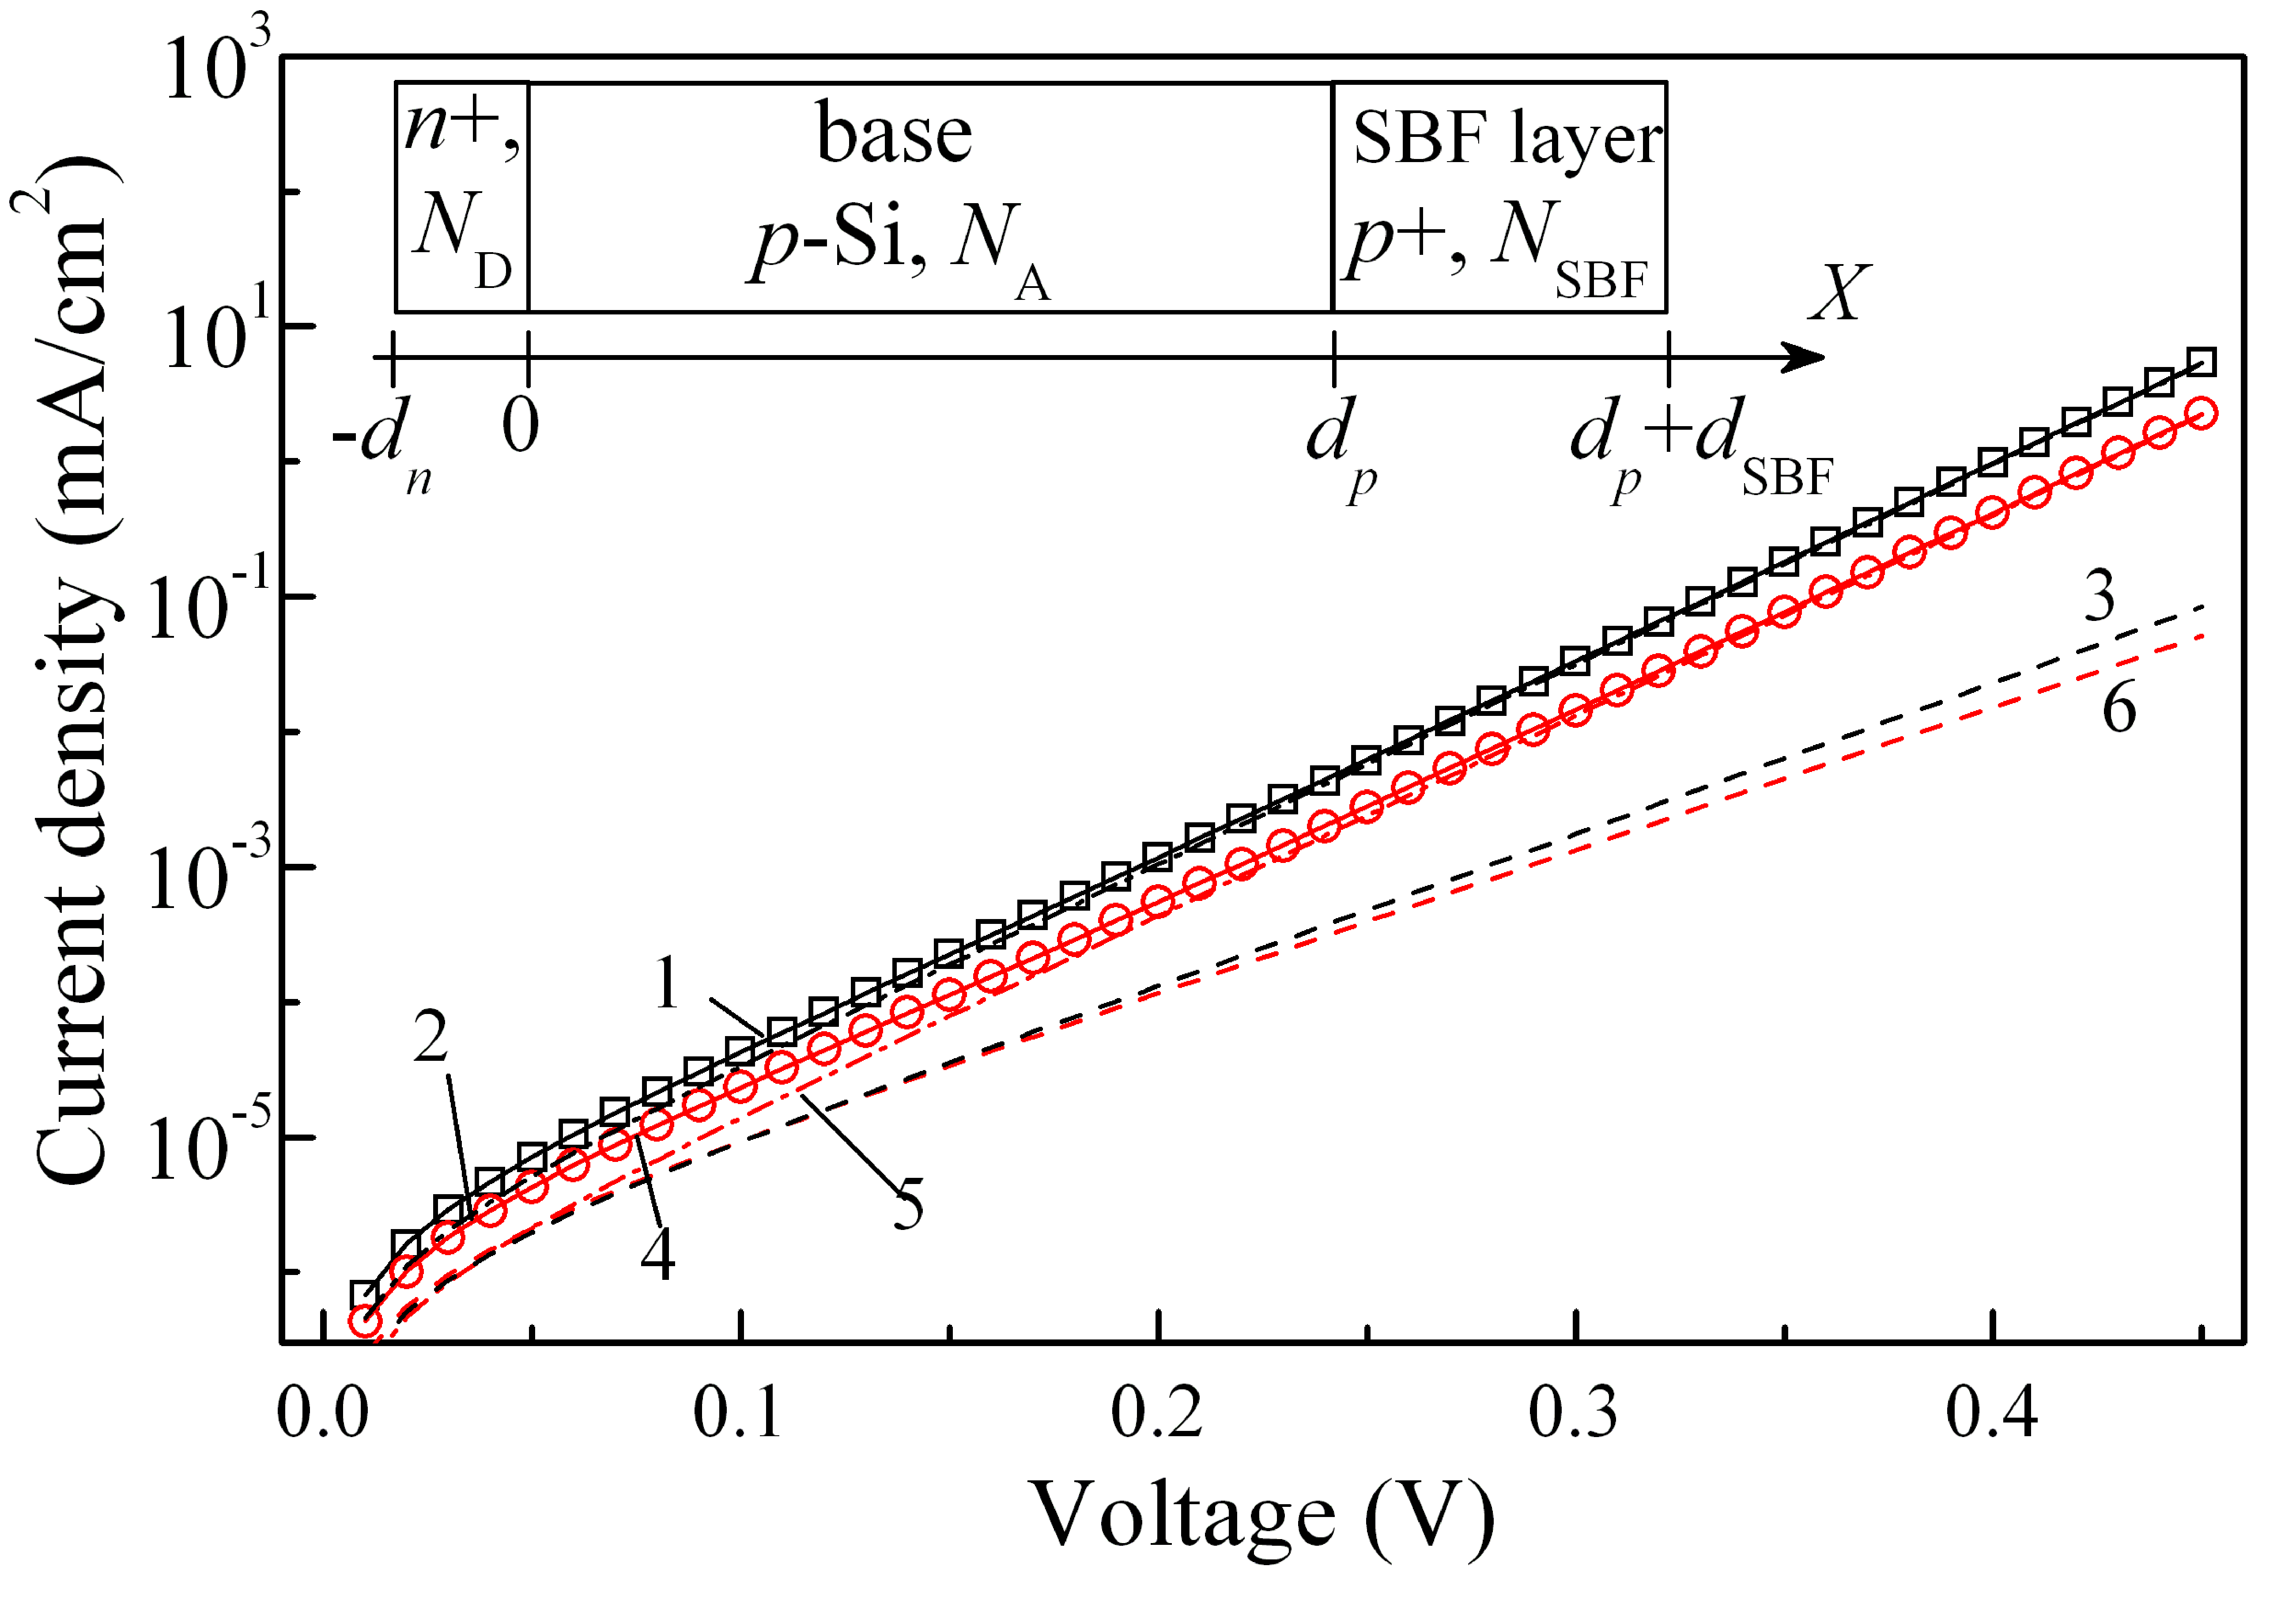
\includegraphics[width=7.5cm]{FigIV}
\caption{.
}
\label{FigIV}
\end{figure}


\begin{figure}
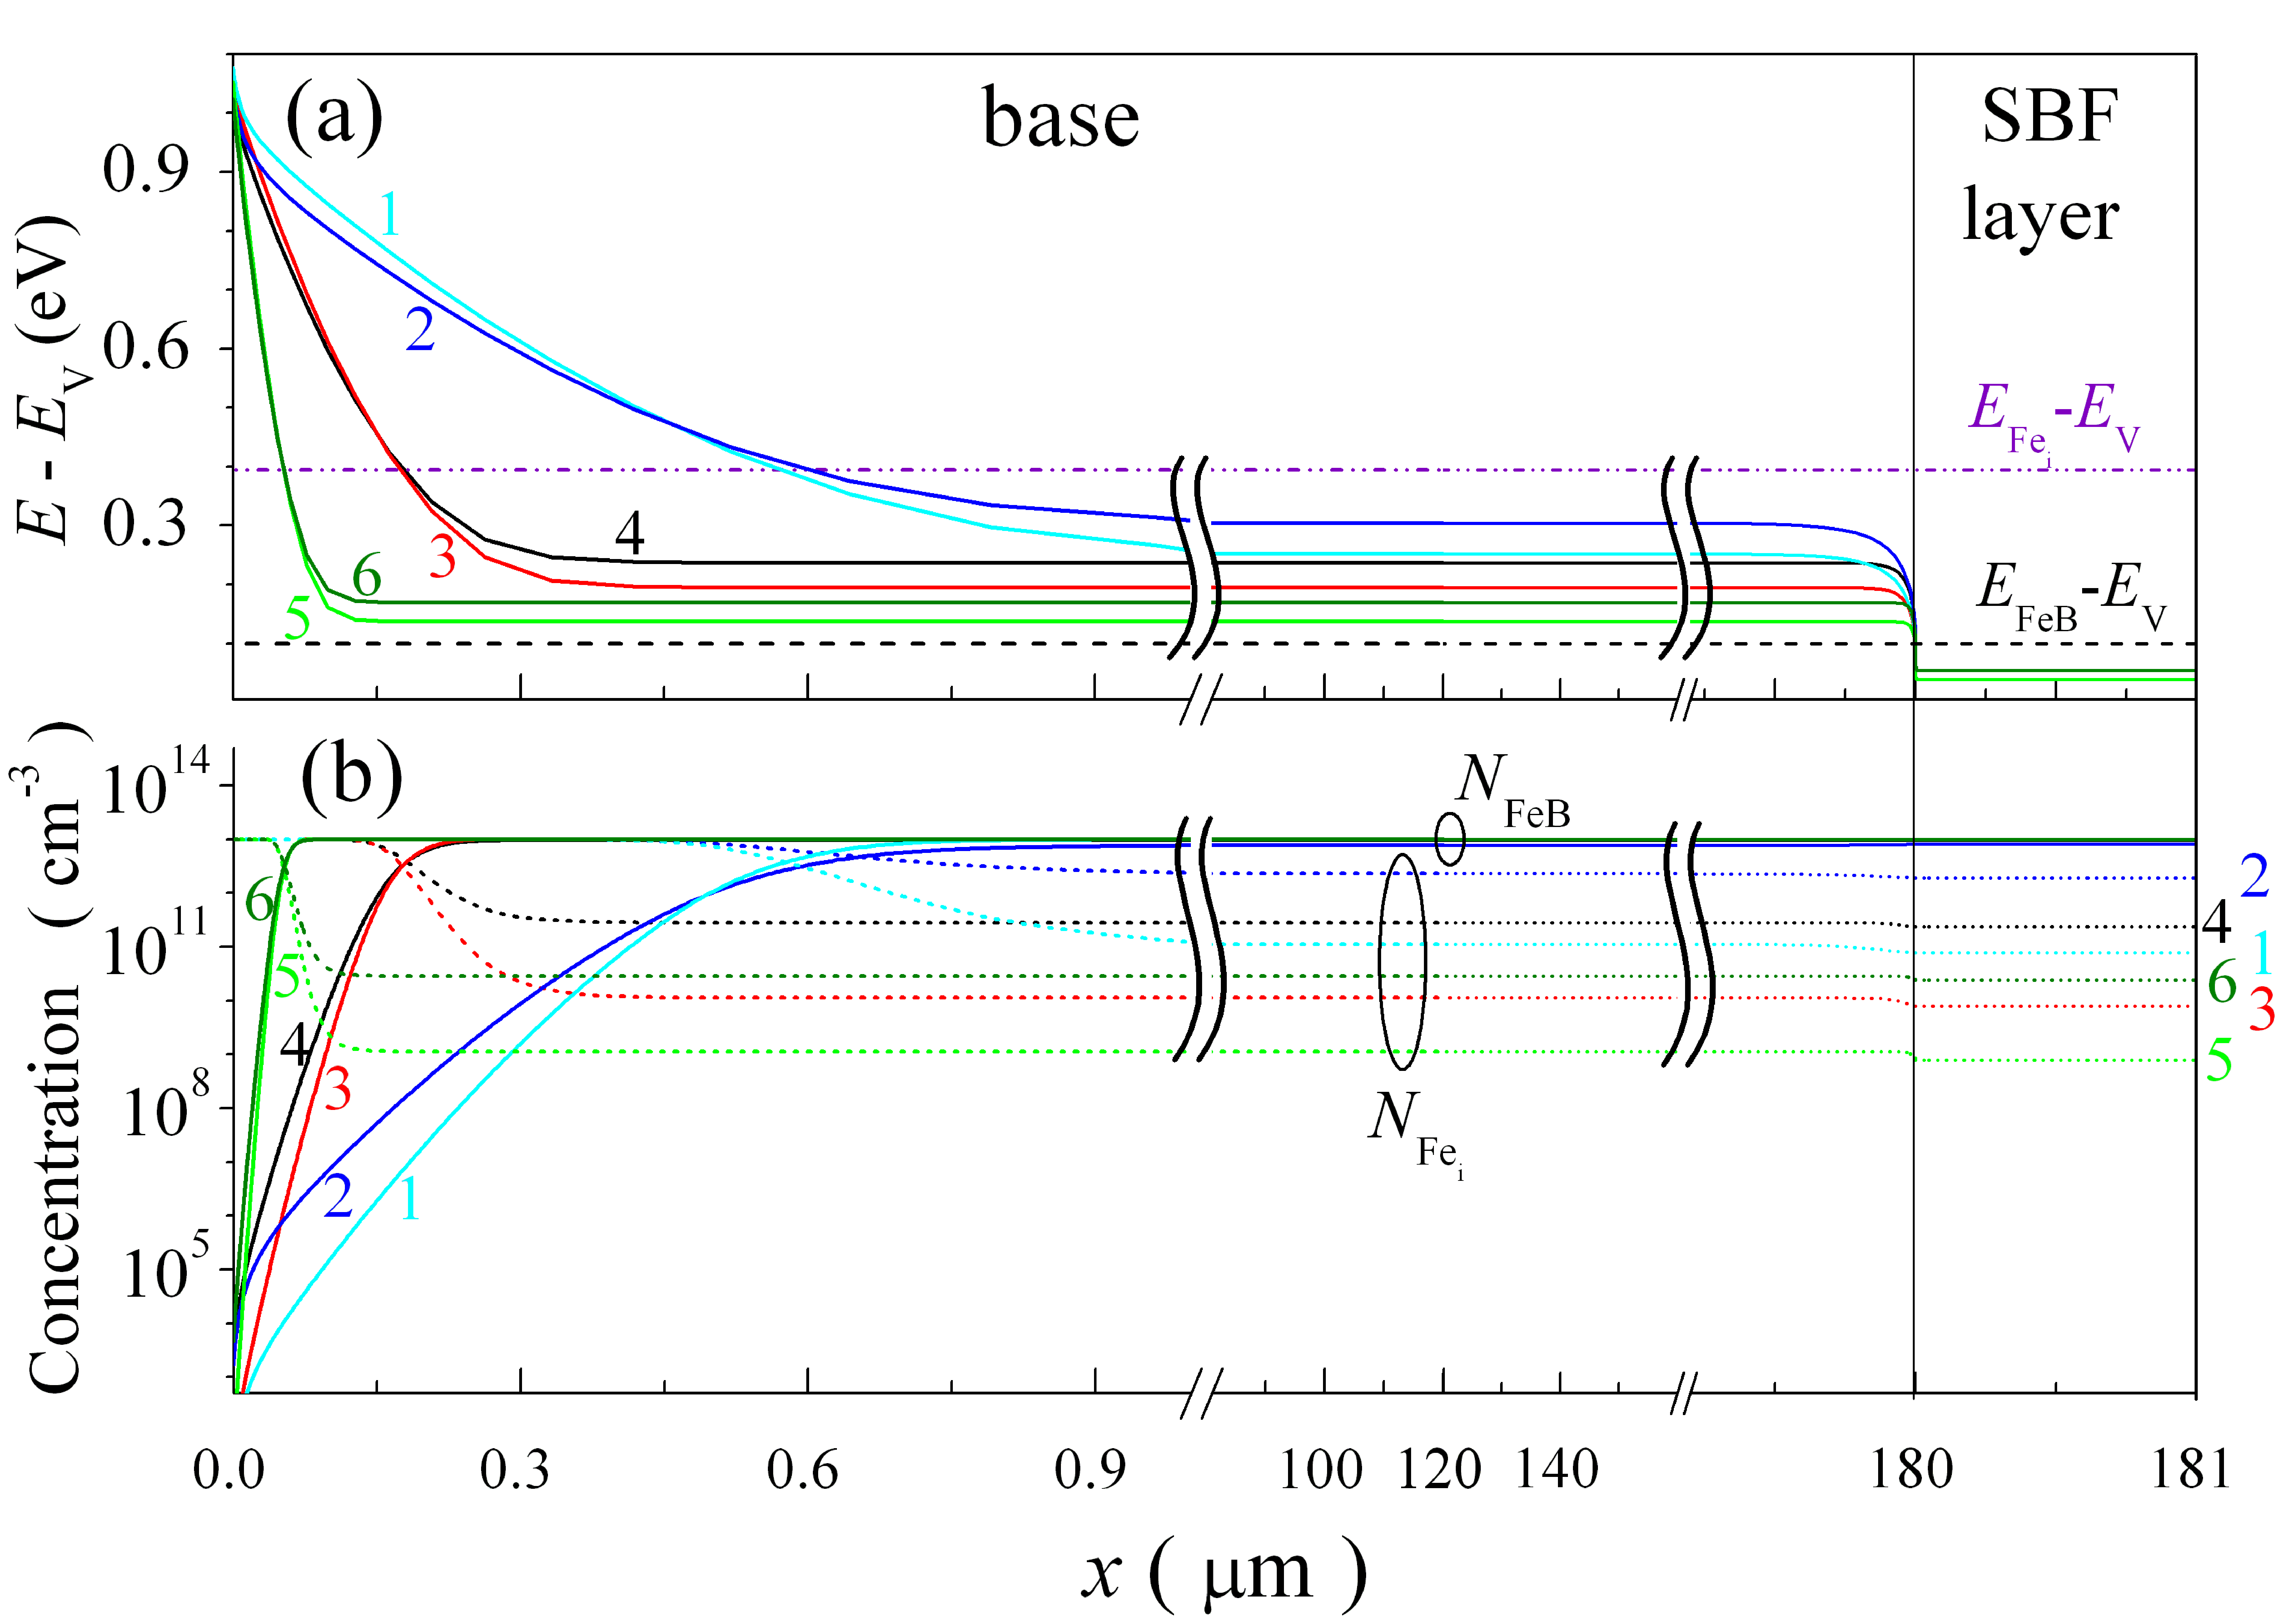
\includegraphics[width=7.5cm]{FigEfAll}
\caption{.
}
\label{FigEf}
\end{figure}

\begin{figure}

\includegraphics[width=7.5cm]{FigFe100d24} \hfill

\includegraphics[width=7.5cm]{FigFe103d24}
\caption{.
}
\label{FigTNa}
\end{figure}

\begin{figure}
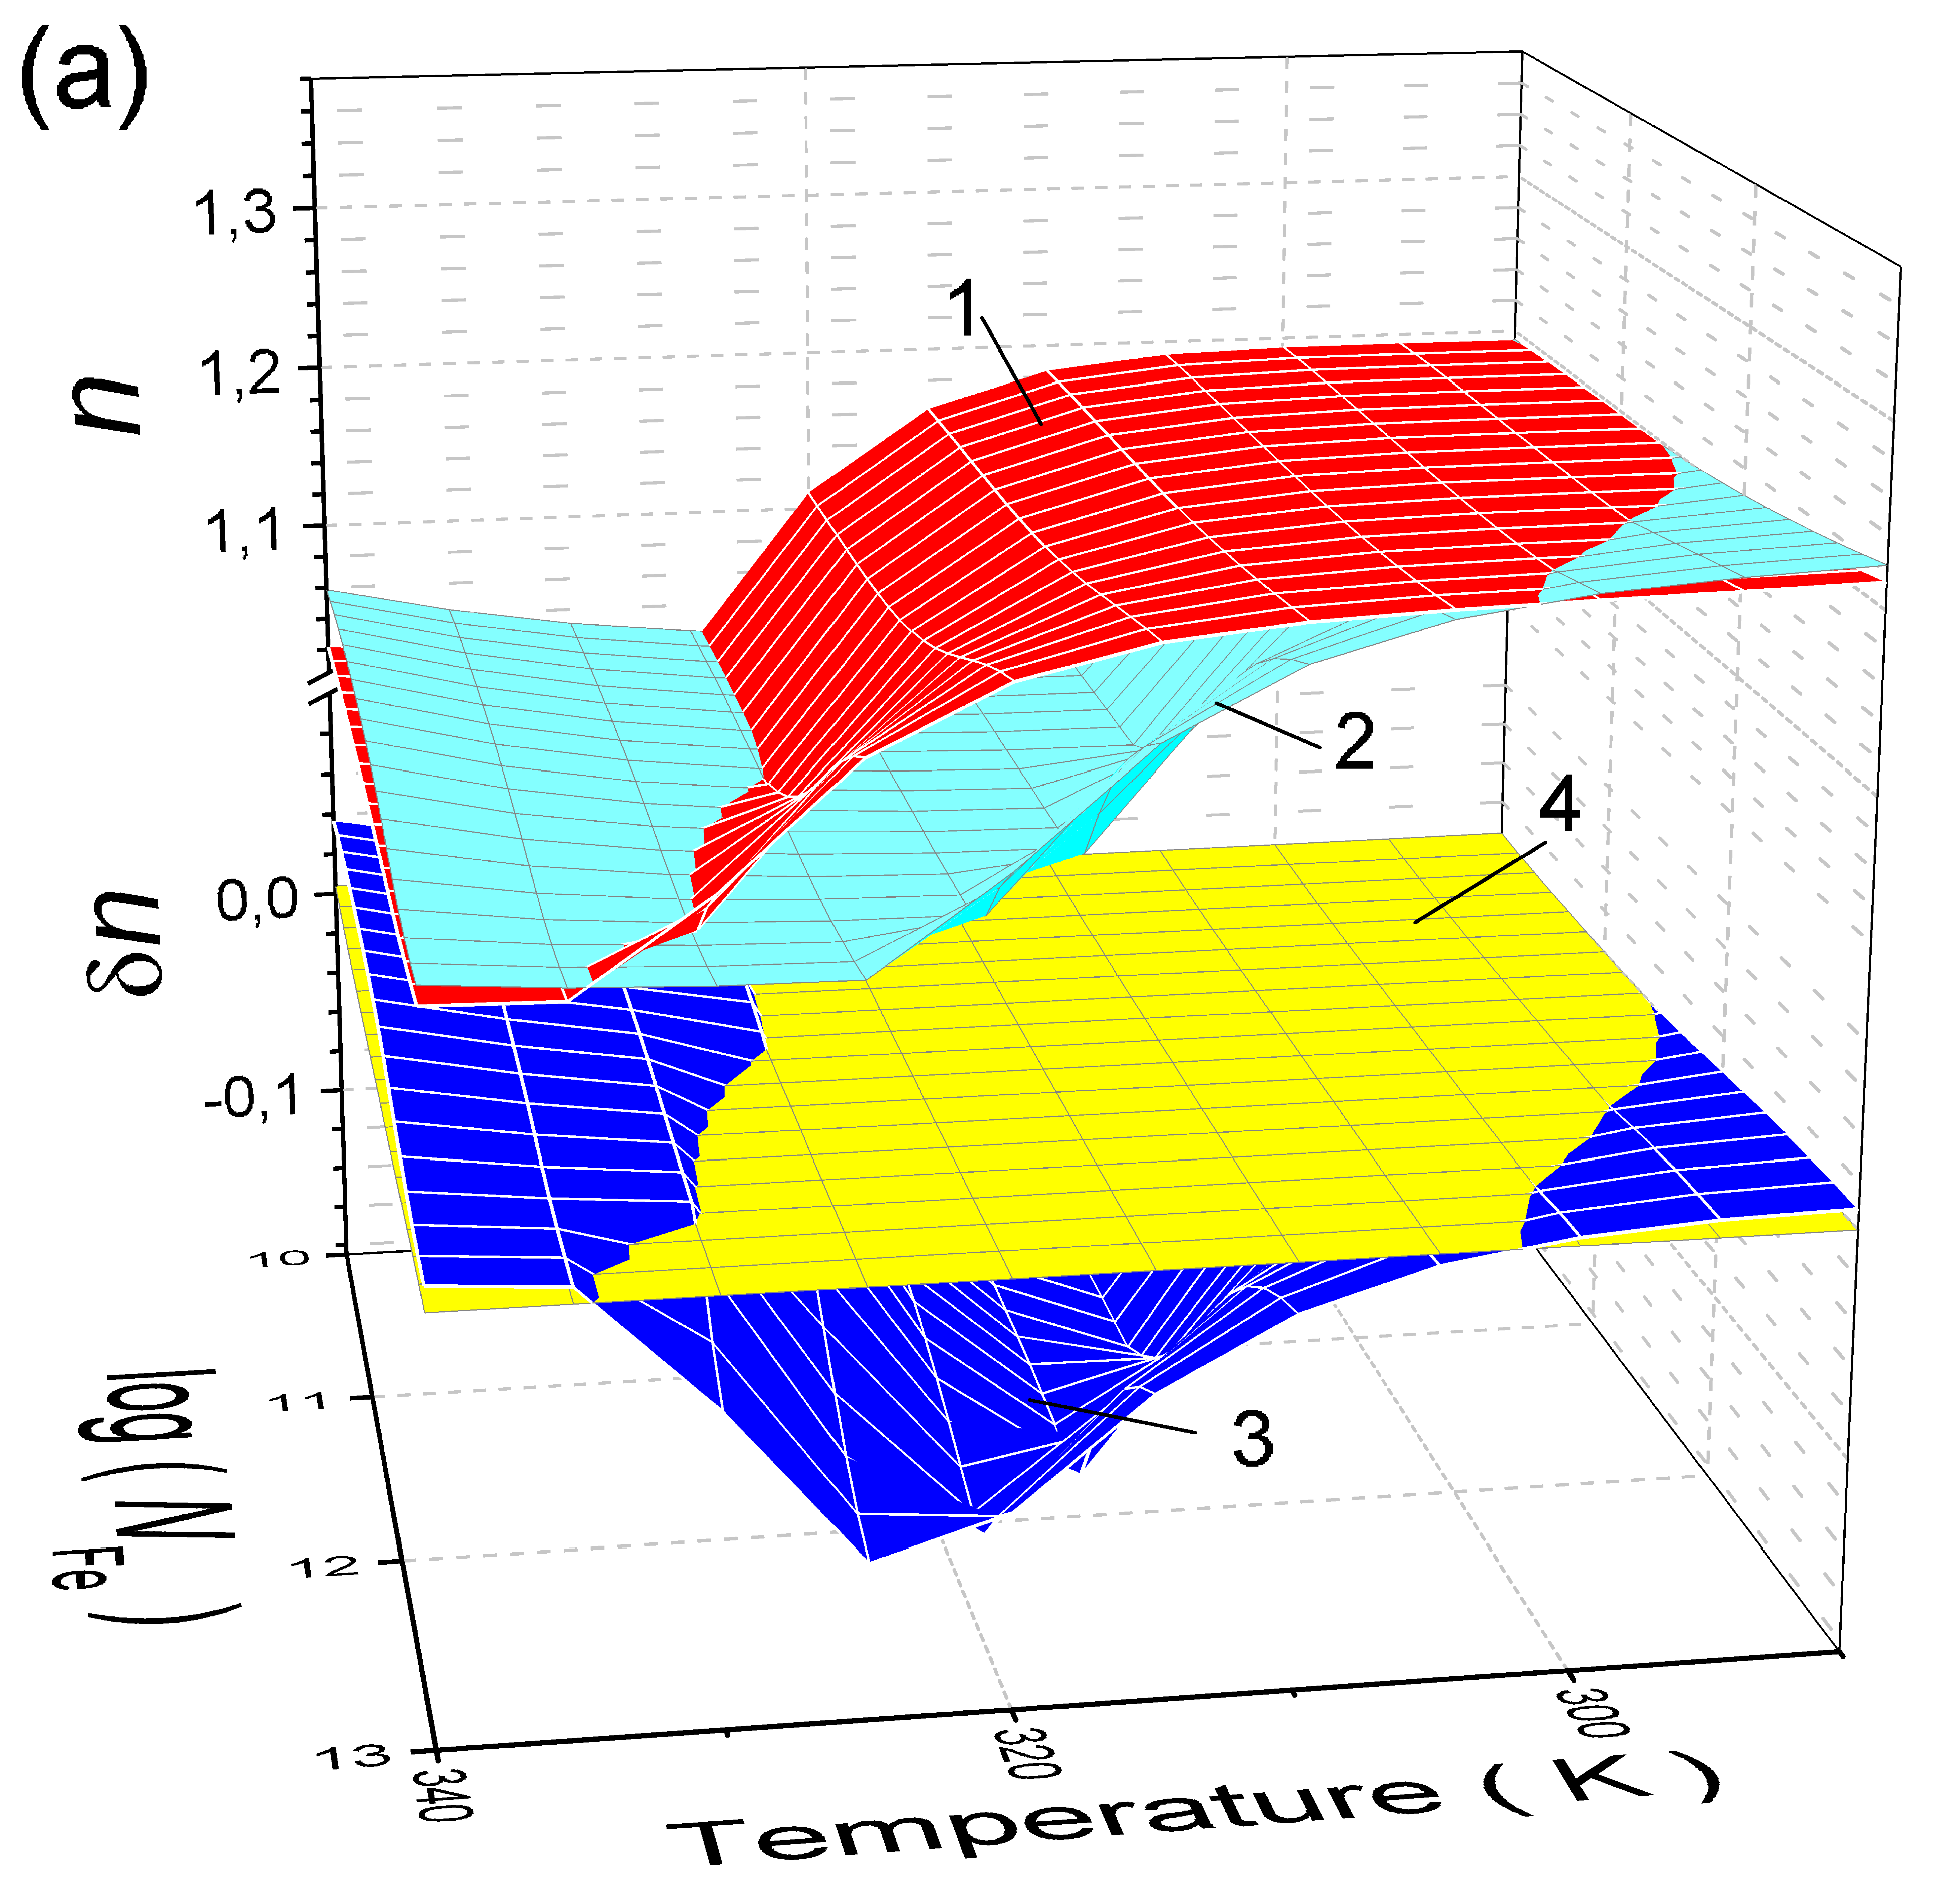
\includegraphics[width=4.9cm]{FigB105d15} \hfill
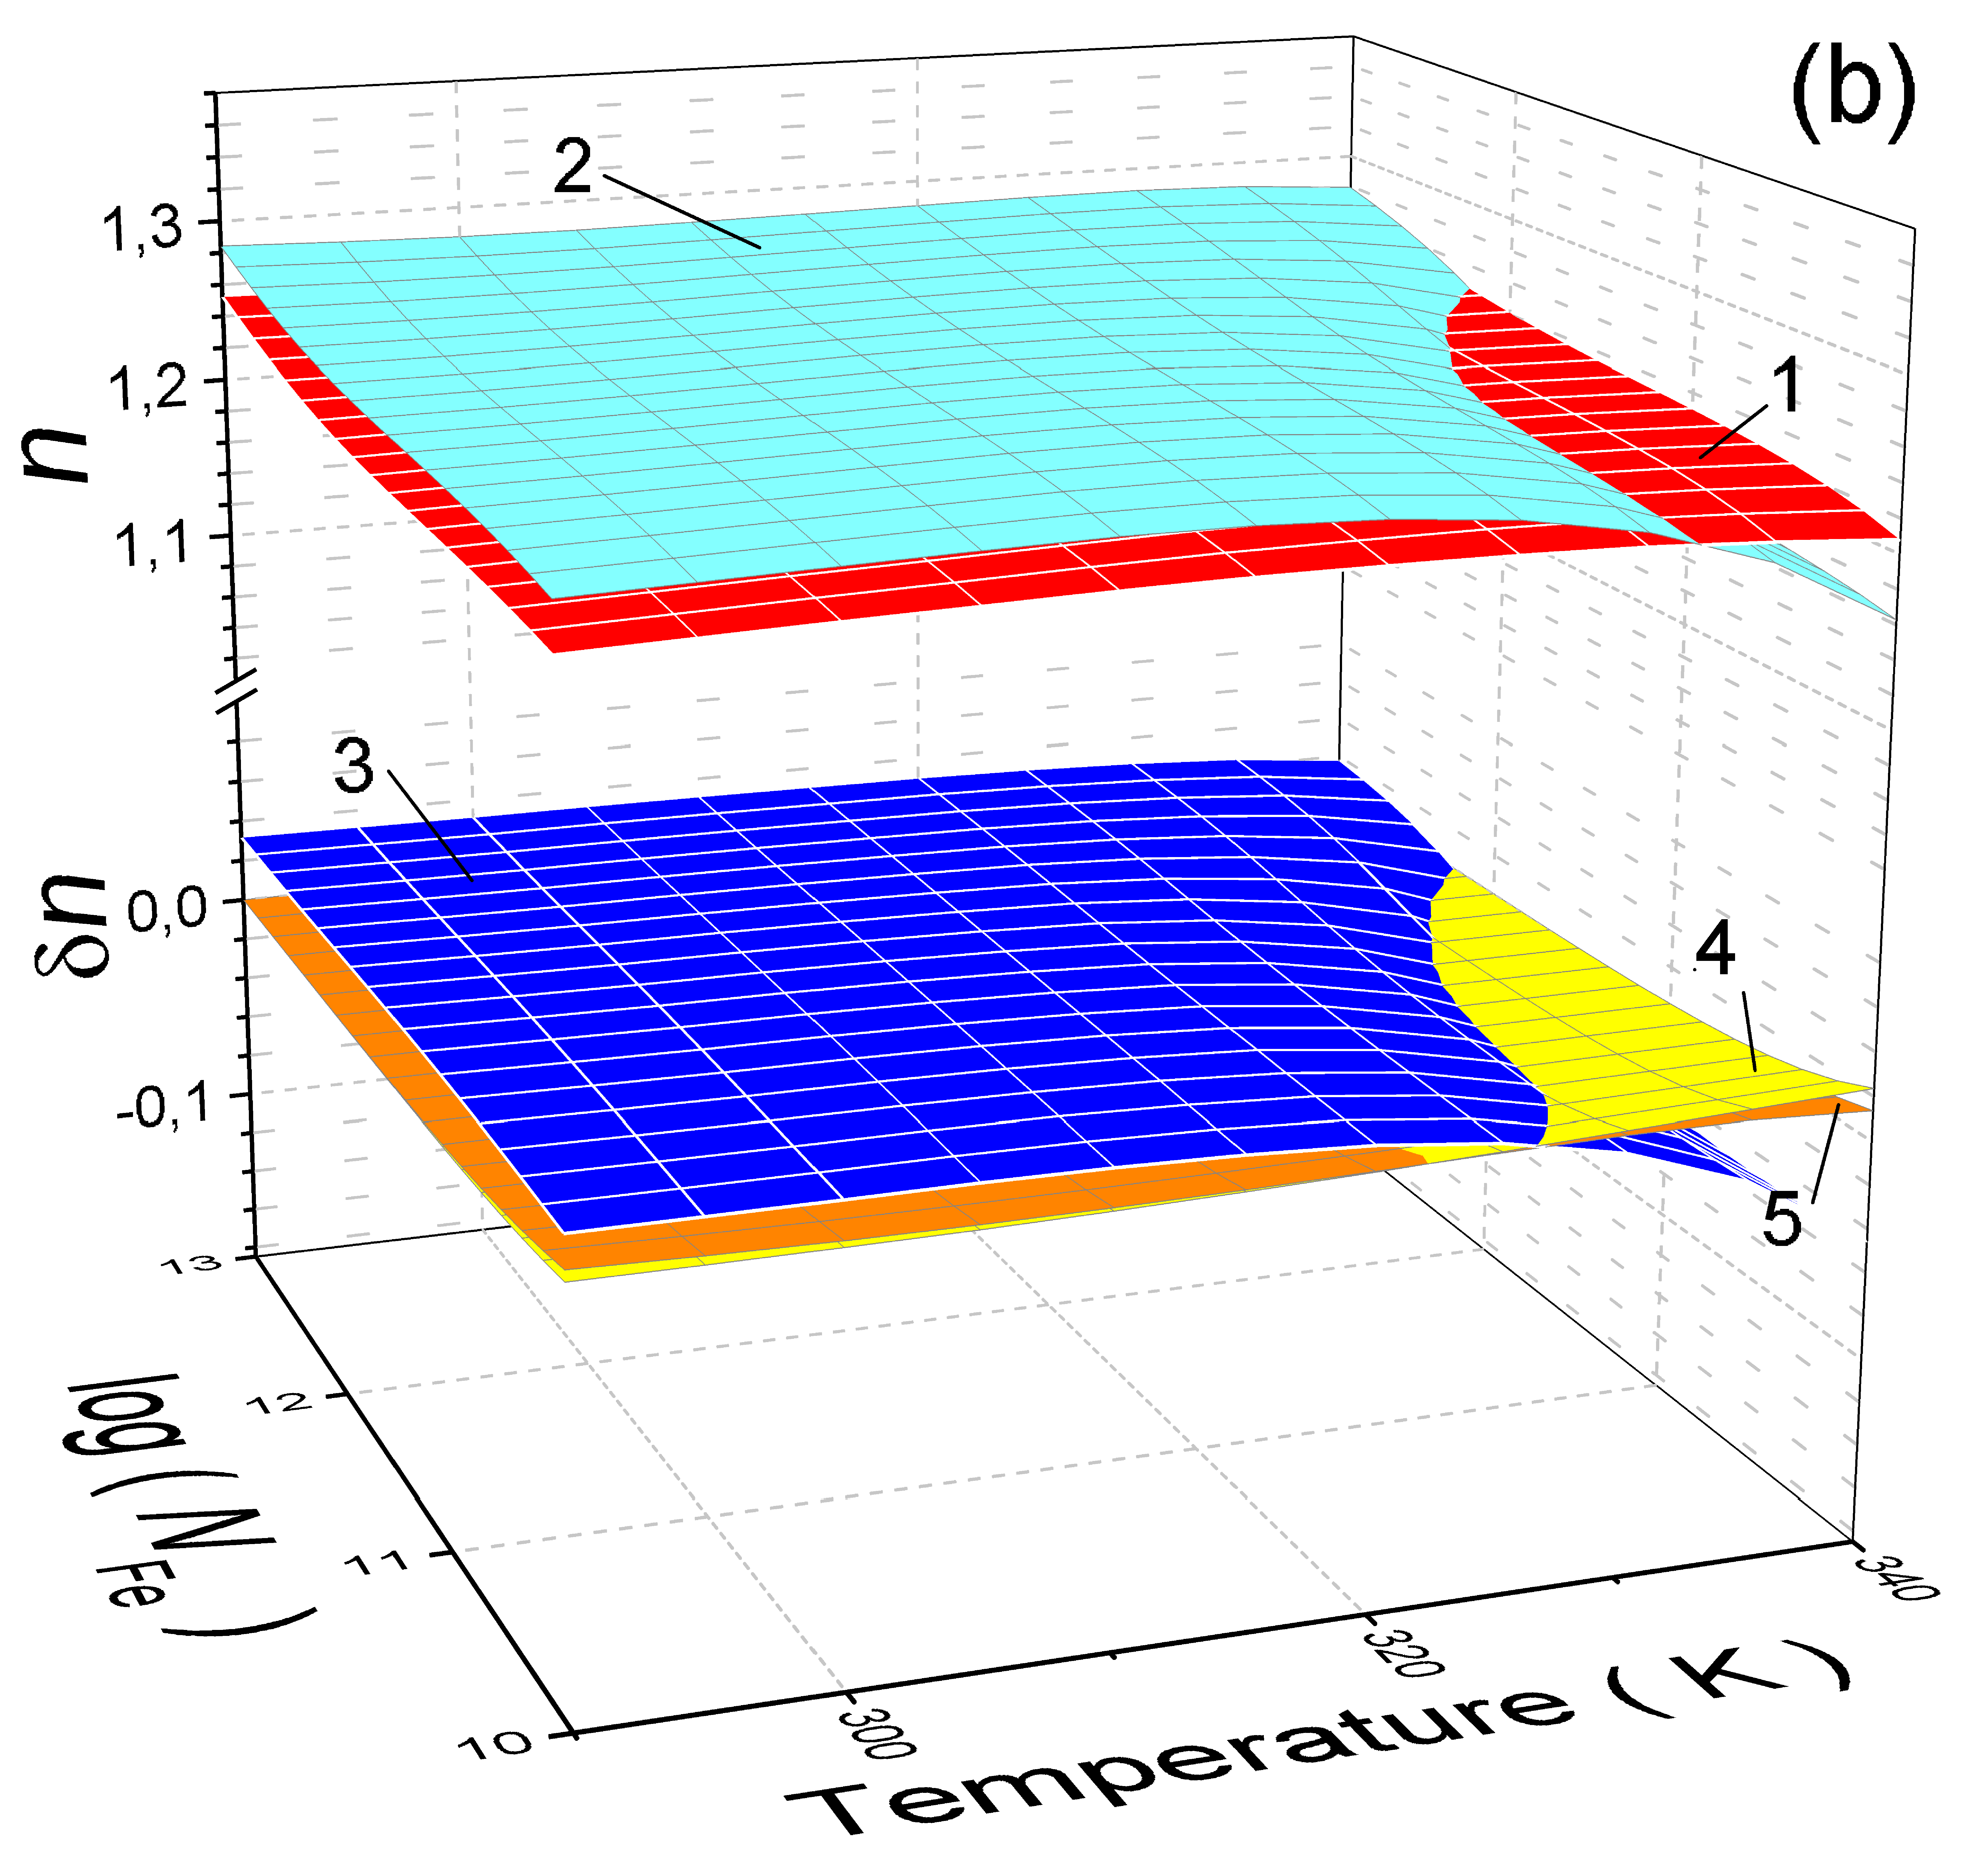
\includegraphics[width=4.9cm]{FigB106d15} \hfill

\includegraphics[width=4.9cm]{FigB107d15}
\caption{.
}
\label{FigTNfe}
\end{figure}

\begin{figure}
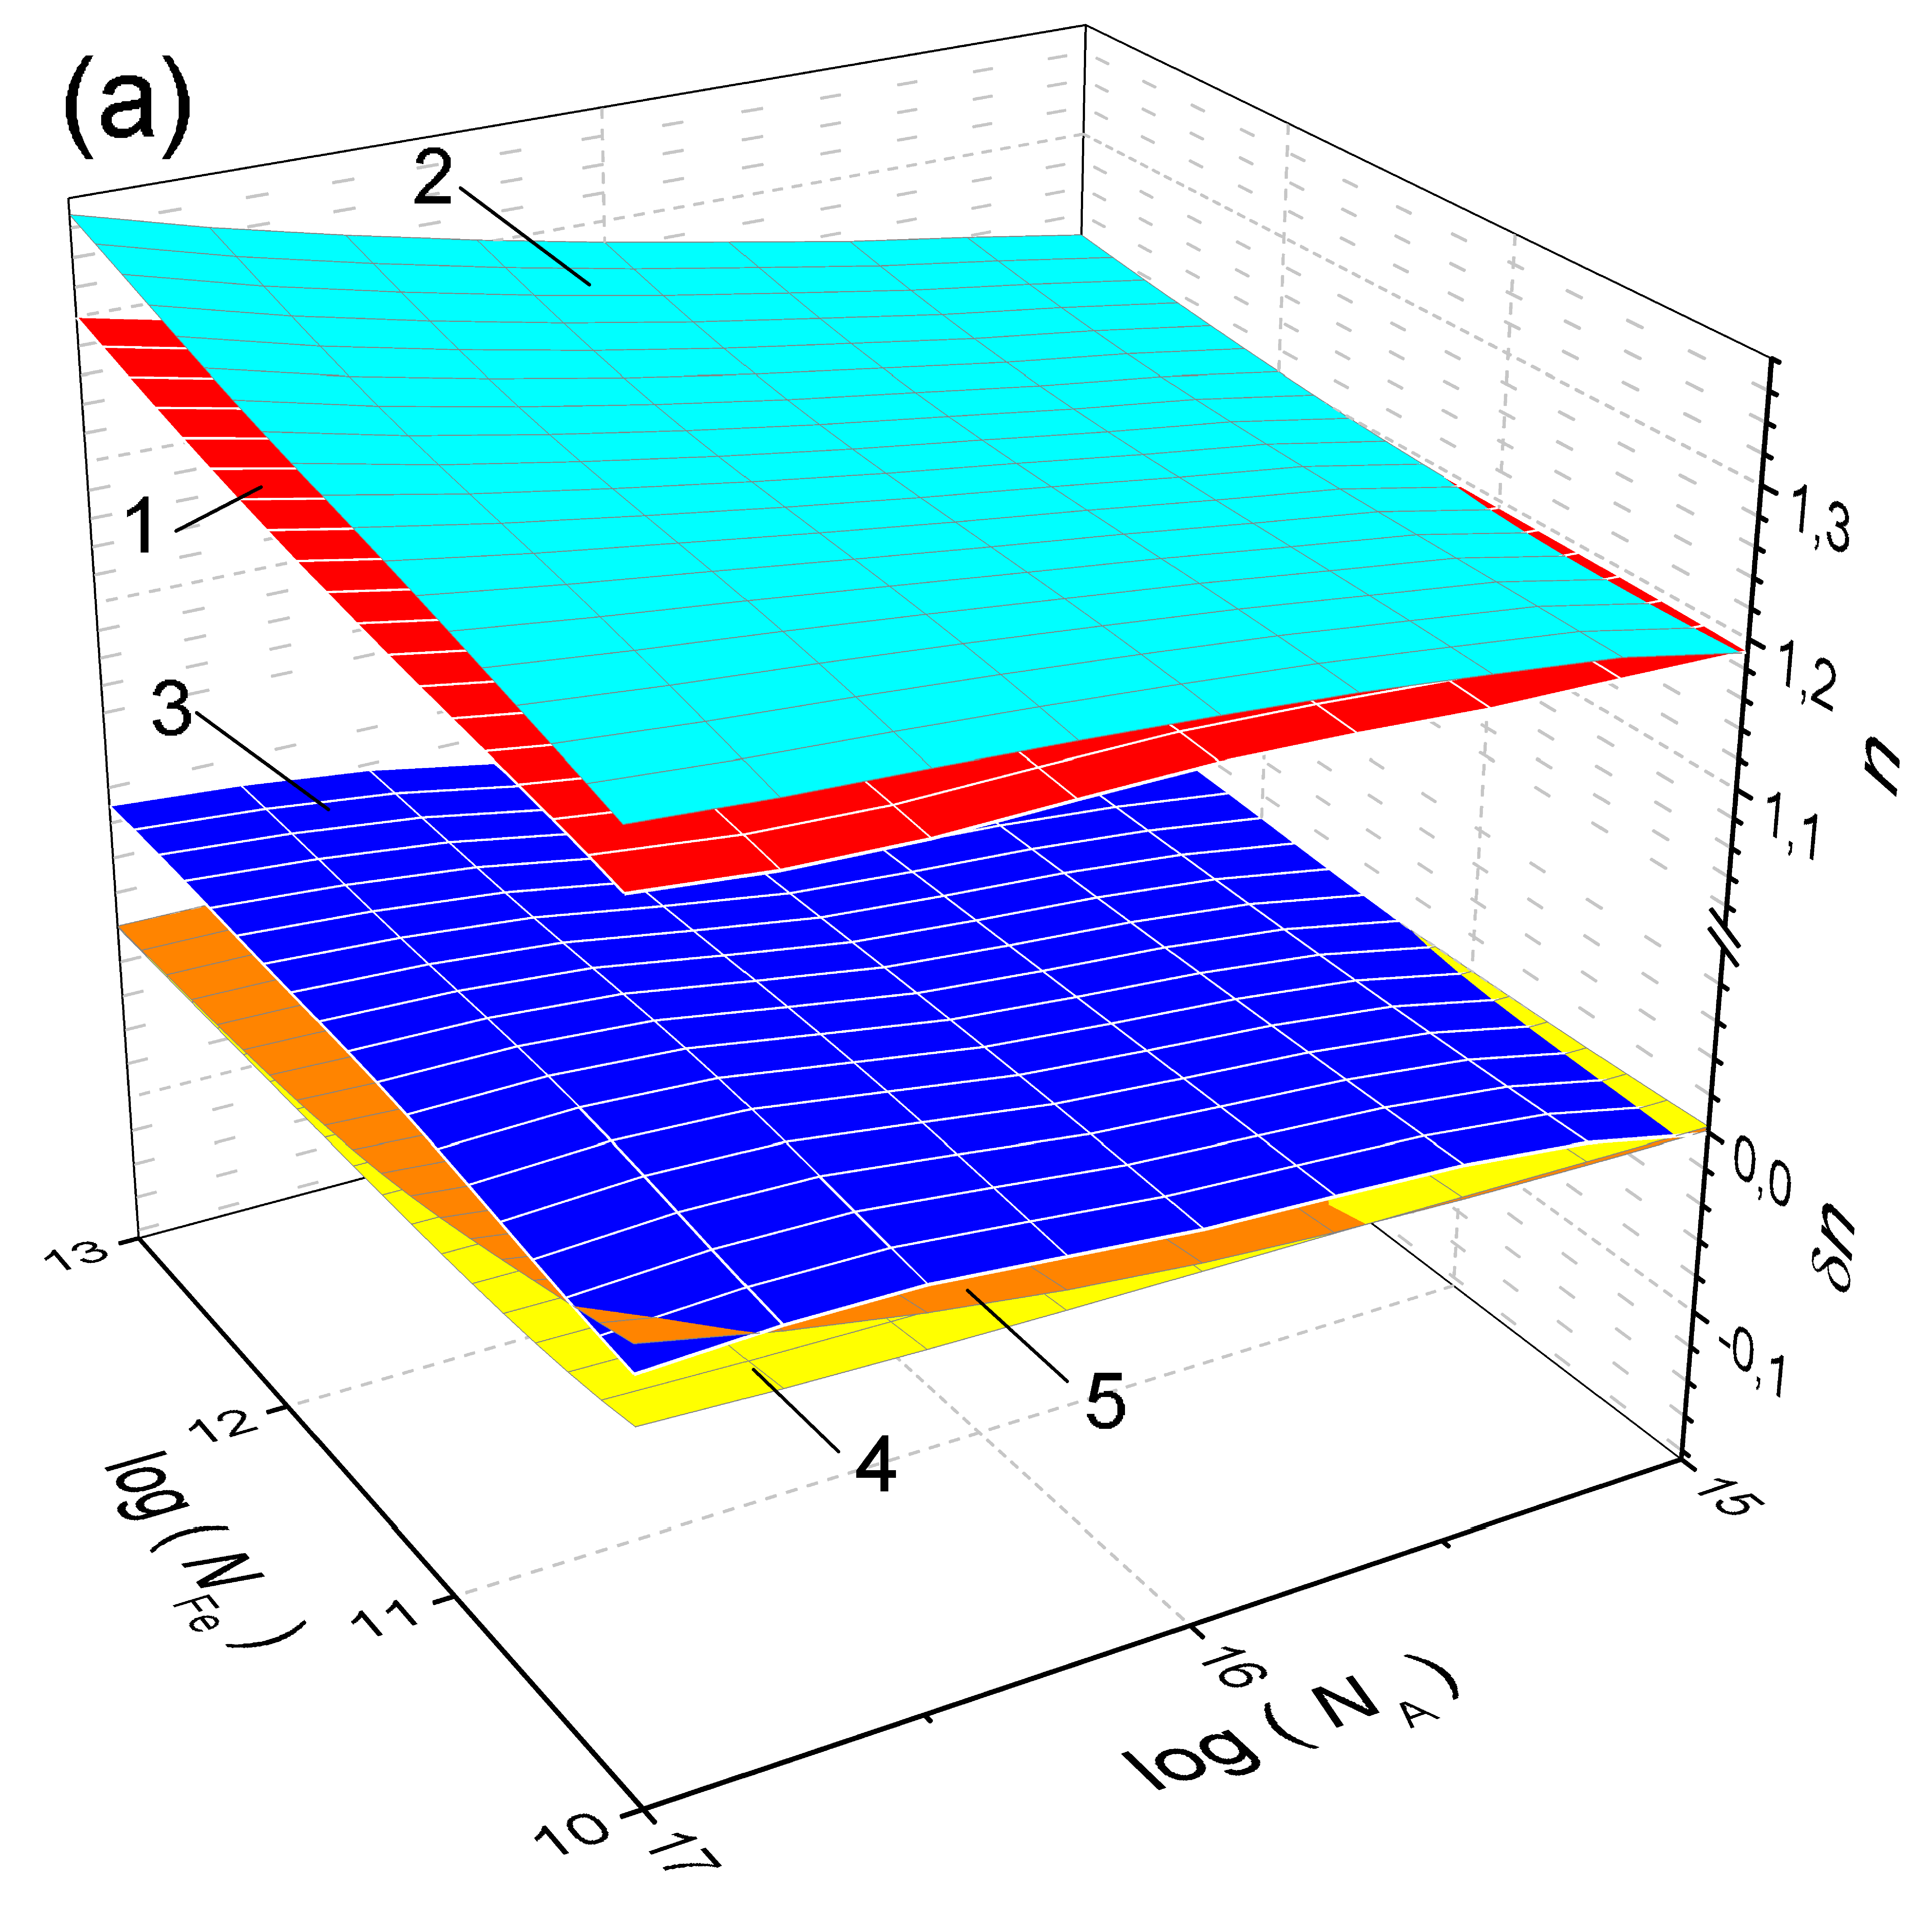
\includegraphics[width=7.5cm]{FigT290d18} \hfill
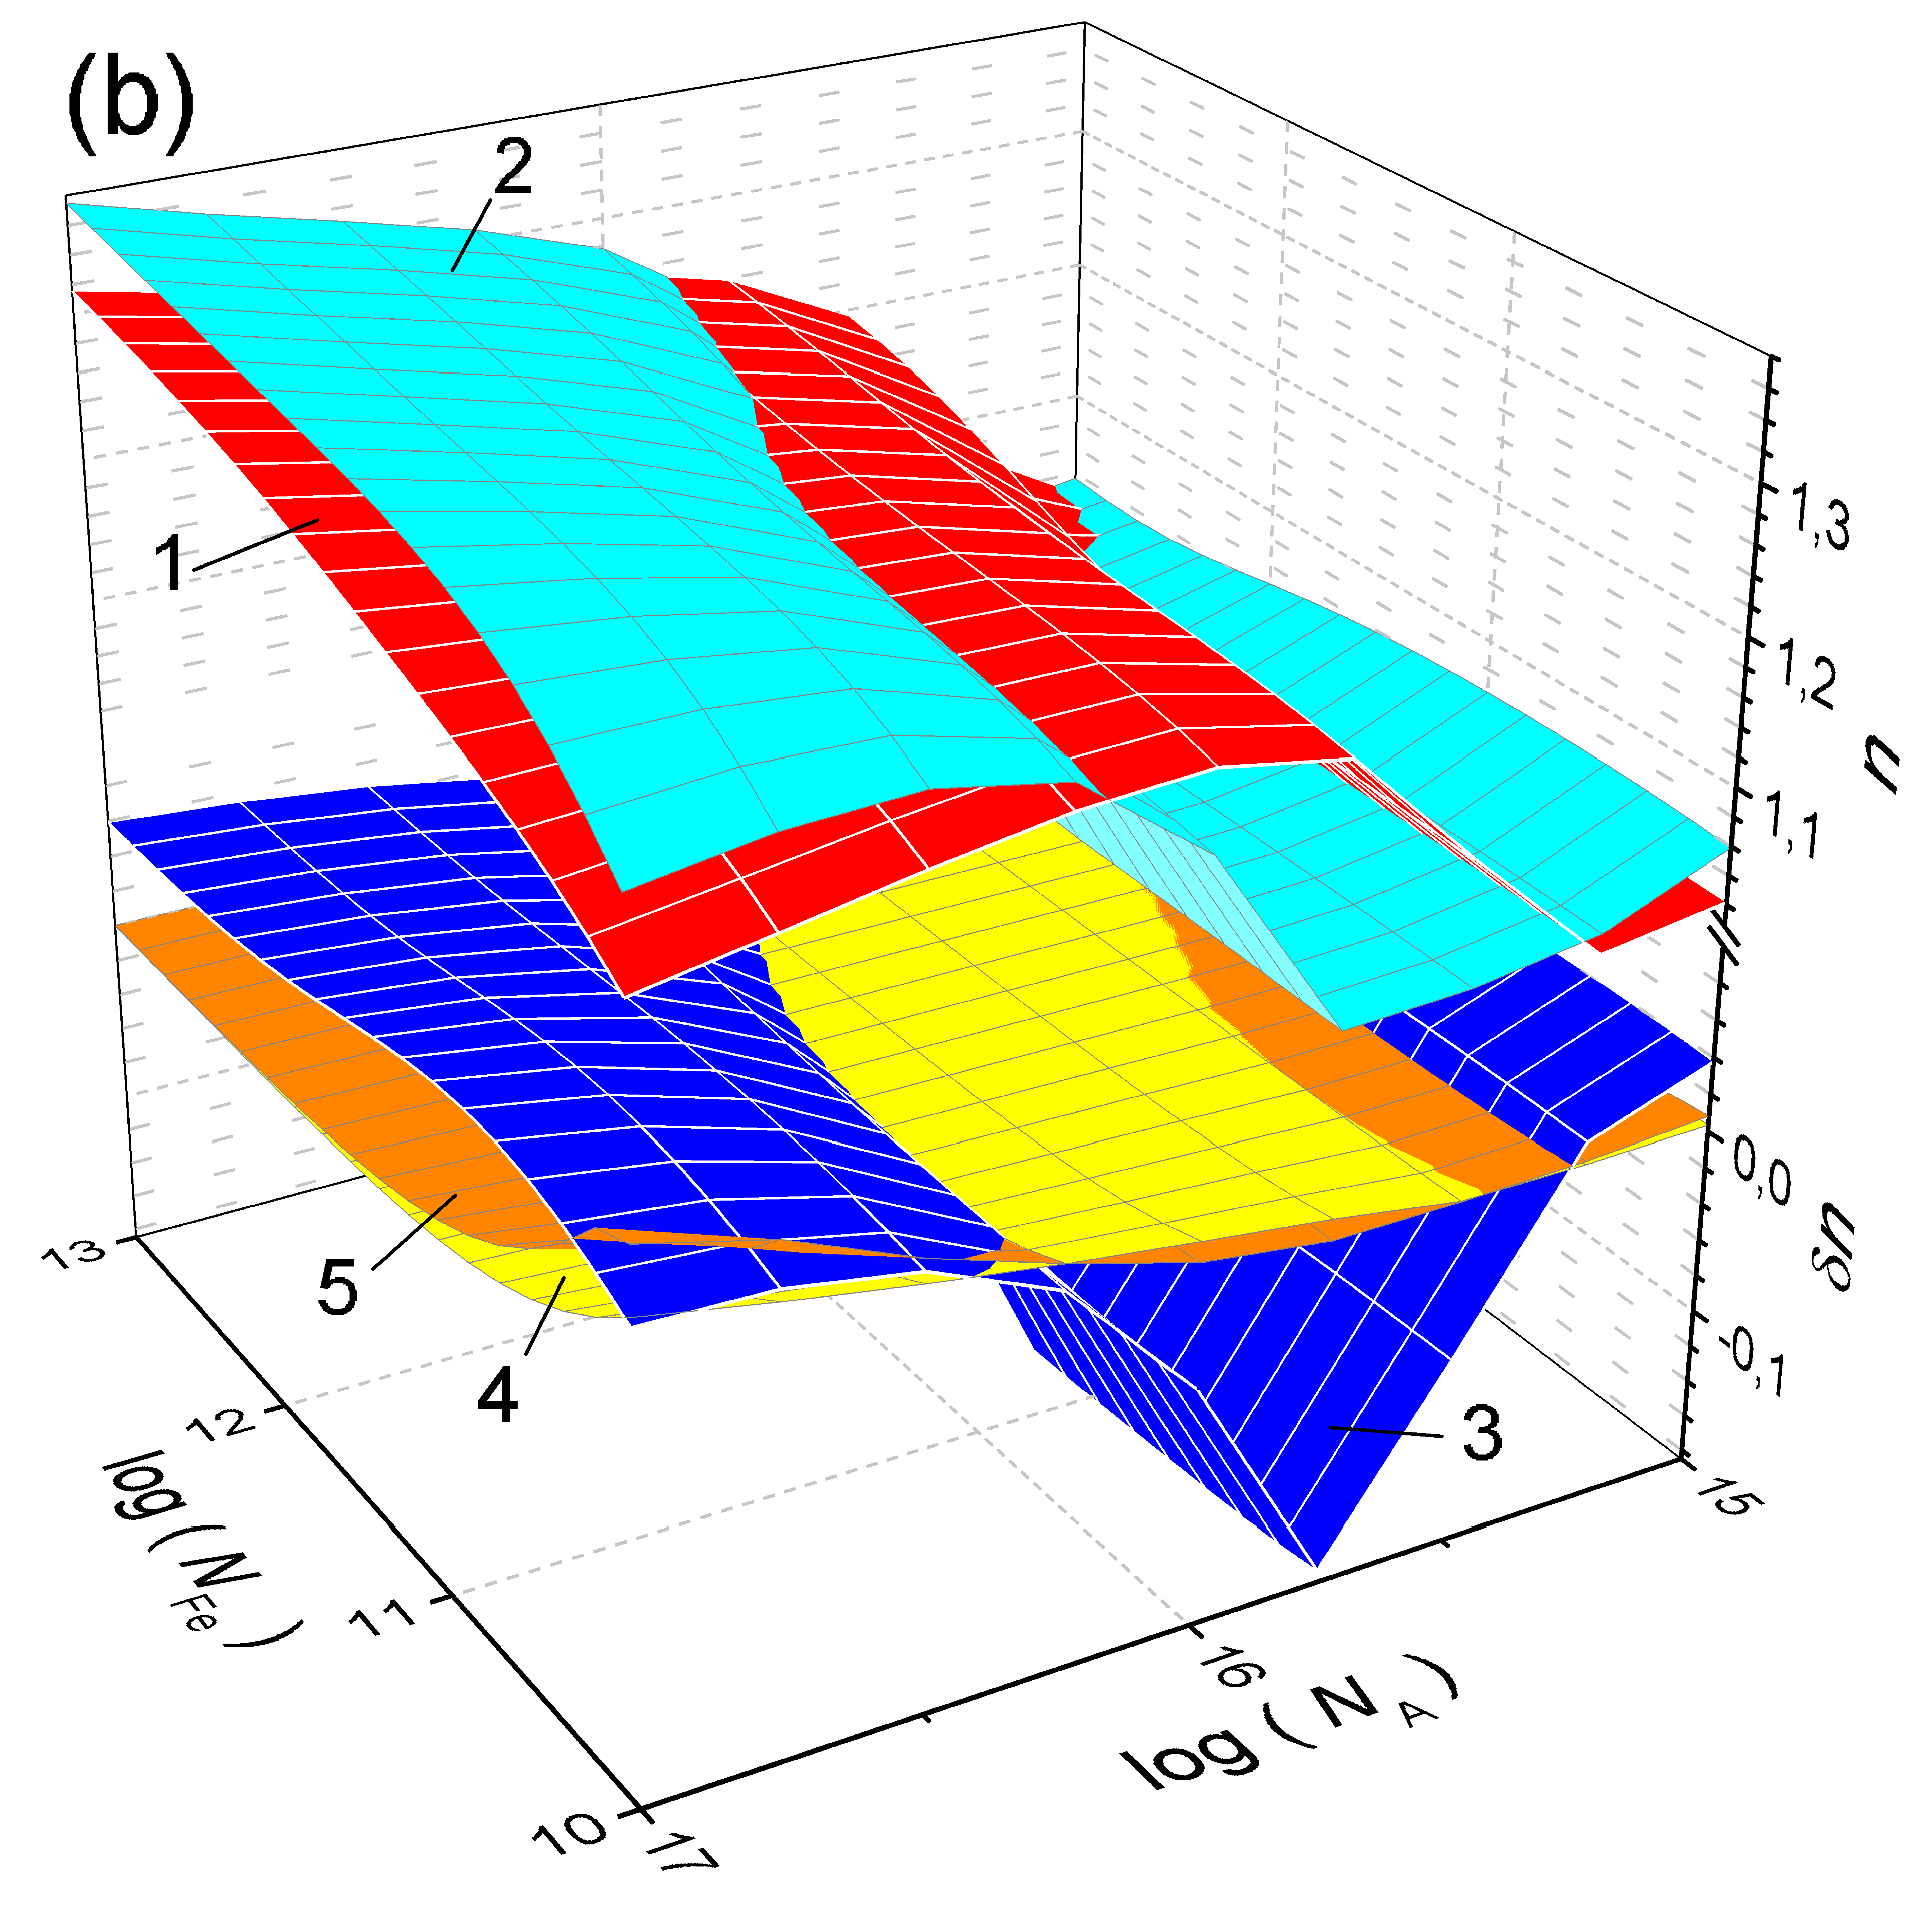
\includegraphics[width=7.5cm]{FigT340d18}
\caption{.
}
\label{FigNaNfe}
\end{figure}

\begin{figure}
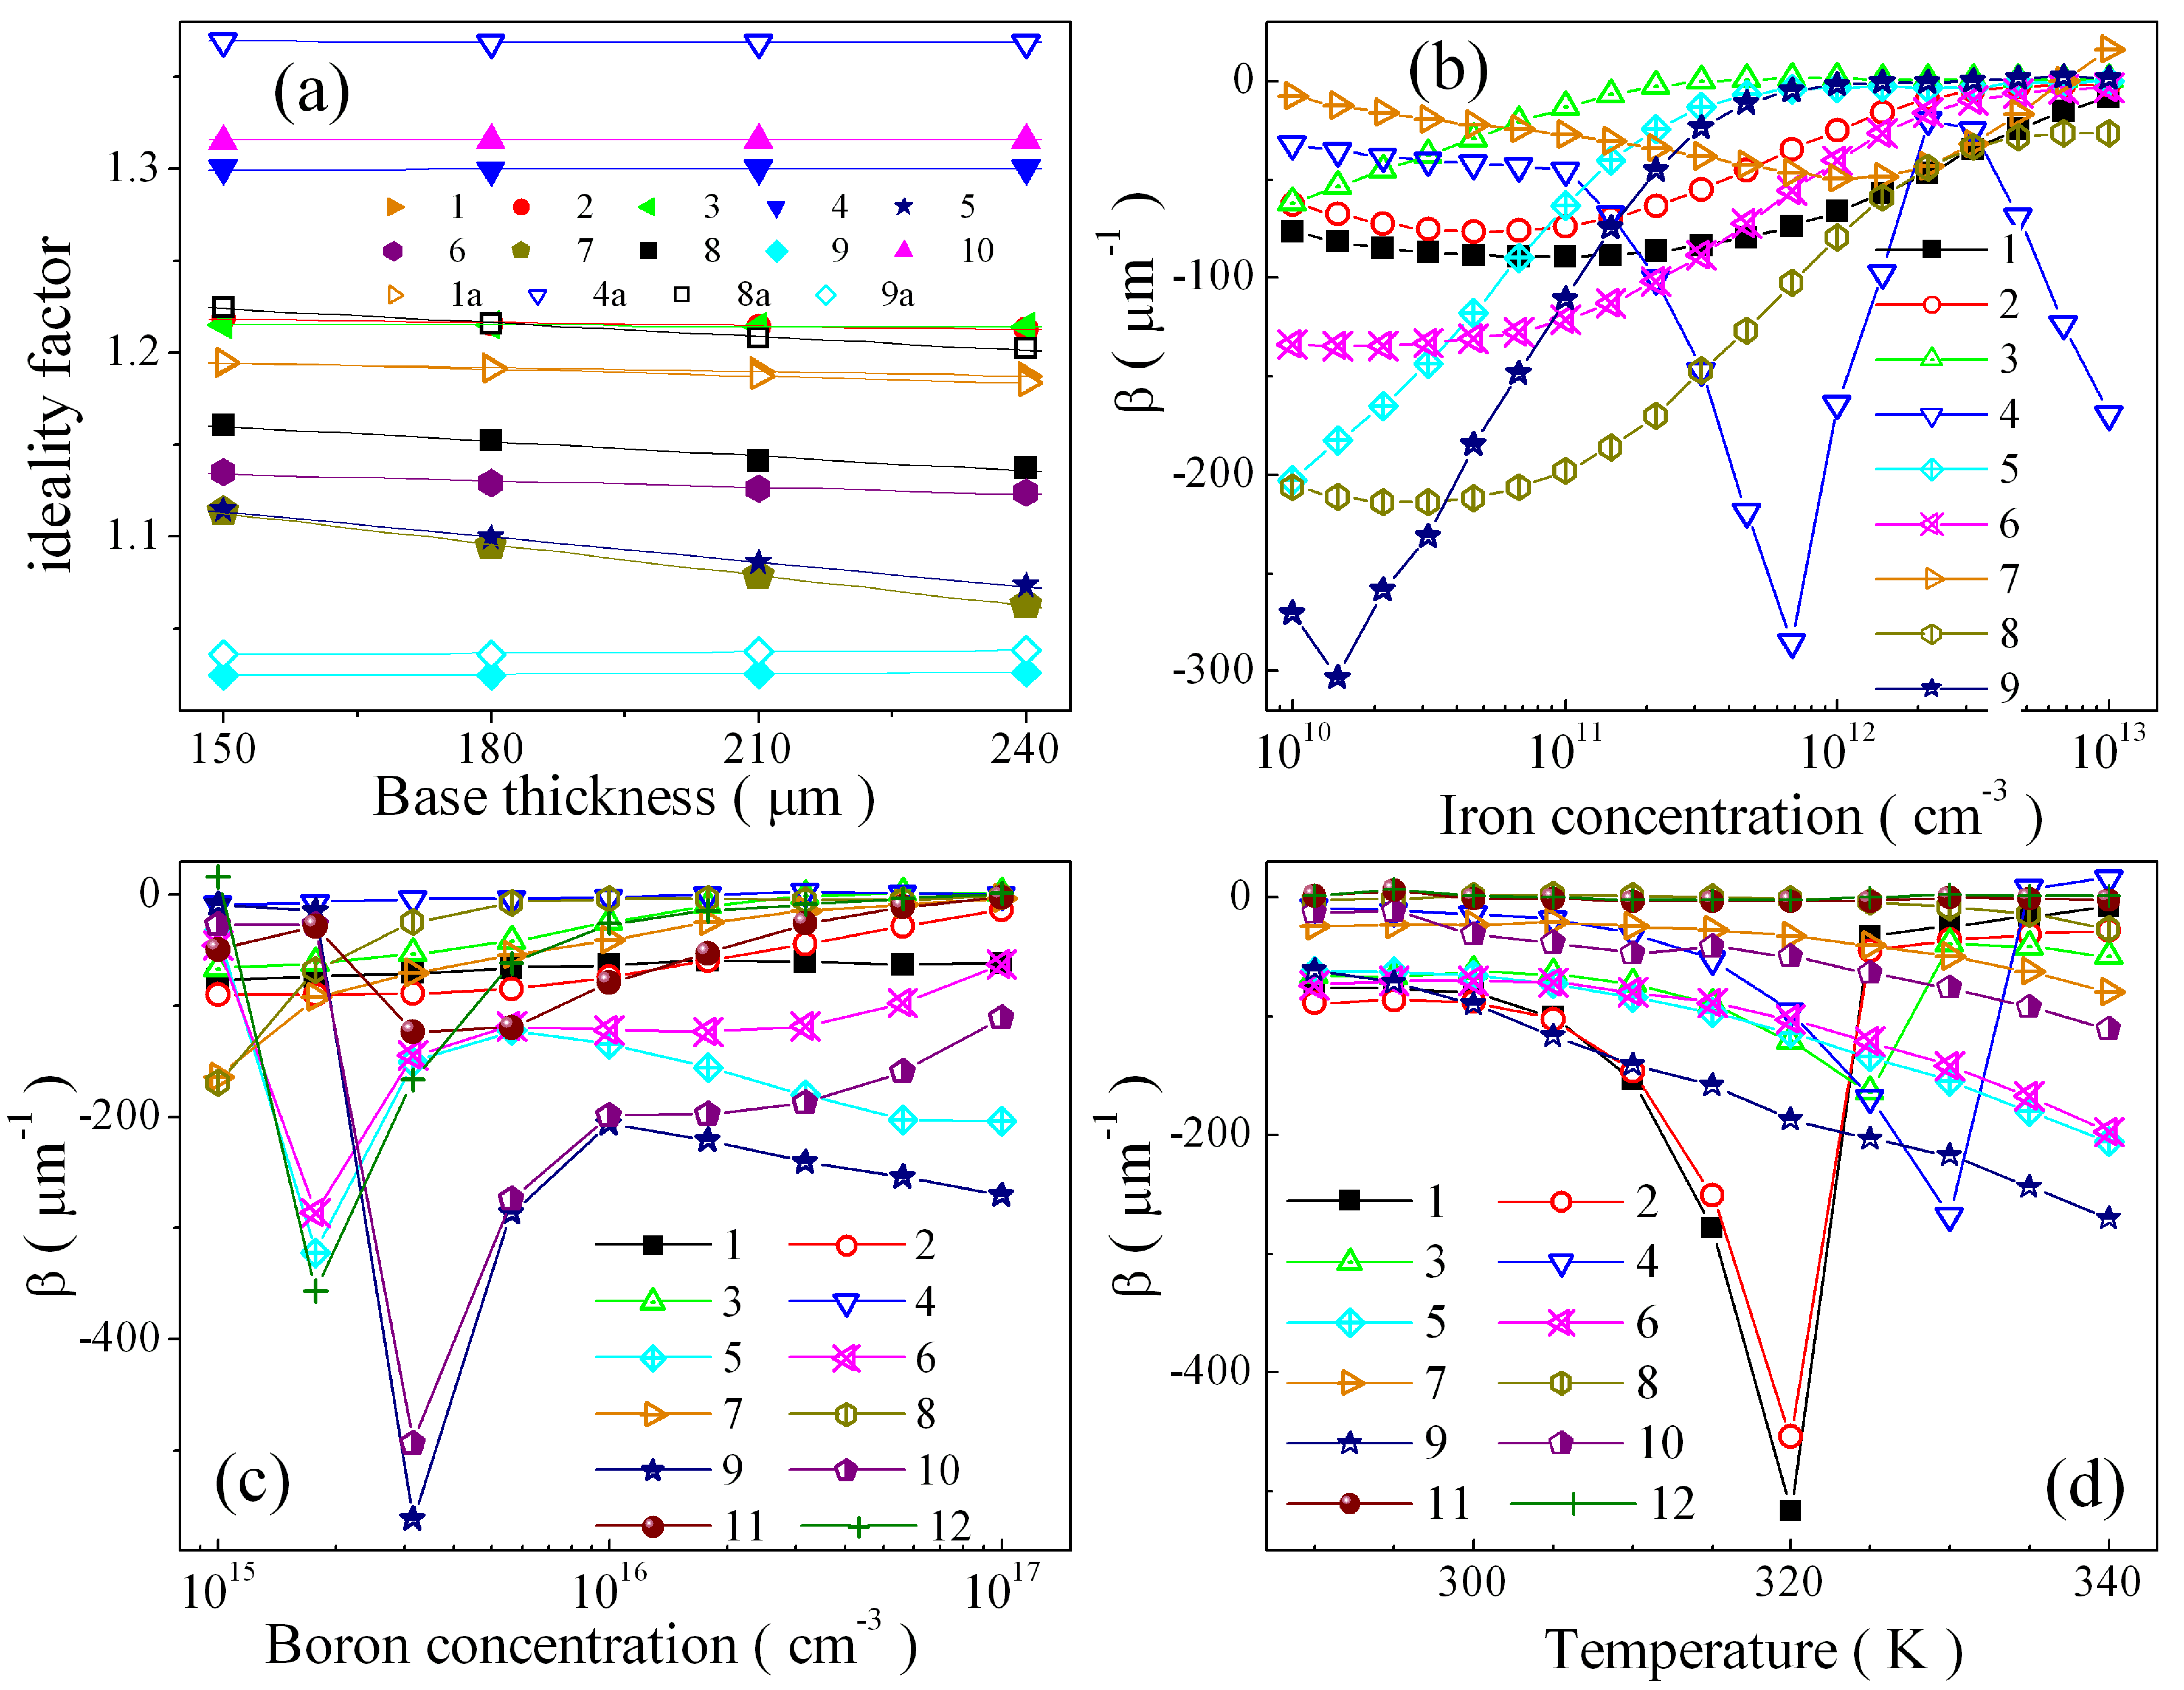
\includegraphics[width=15cm]{FigTotal}
\caption{.
}
\label{FigTotal}
\end{figure}


\begin{figure}
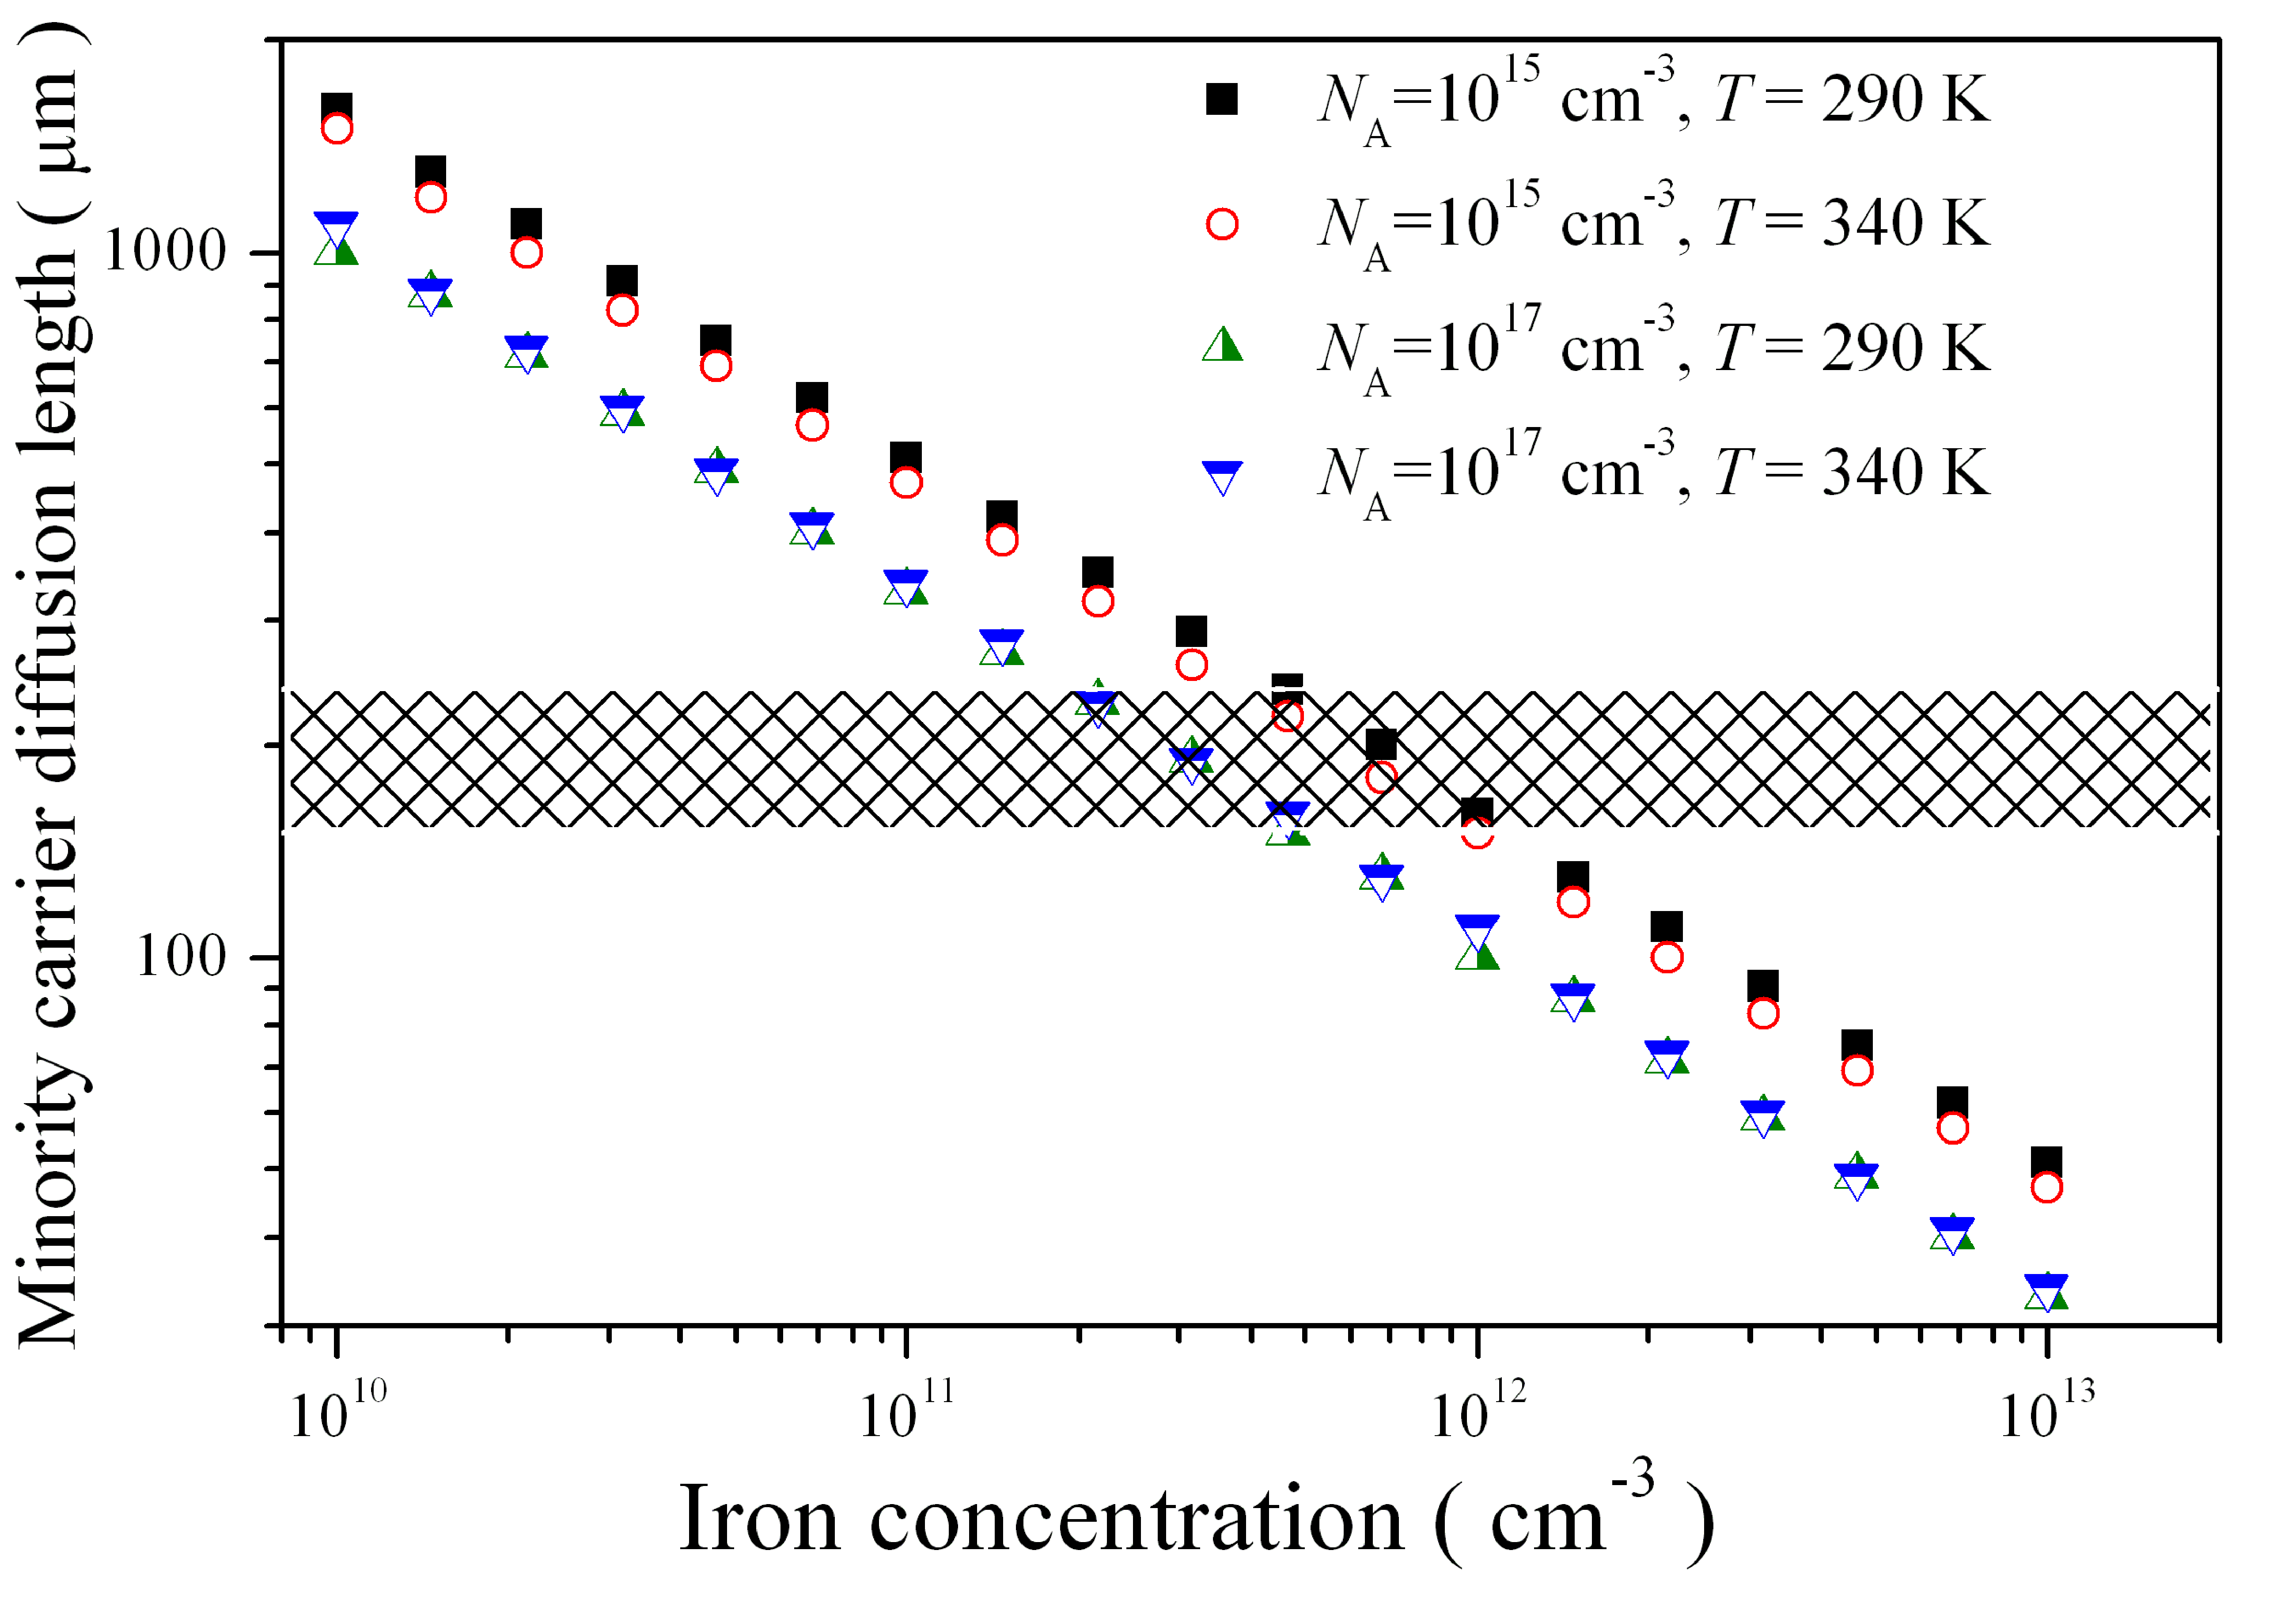
\includegraphics[width=7.5cm]{FigLn}
\caption{.
}
\label{FigLn}
\end{figure}

\begin{figure}
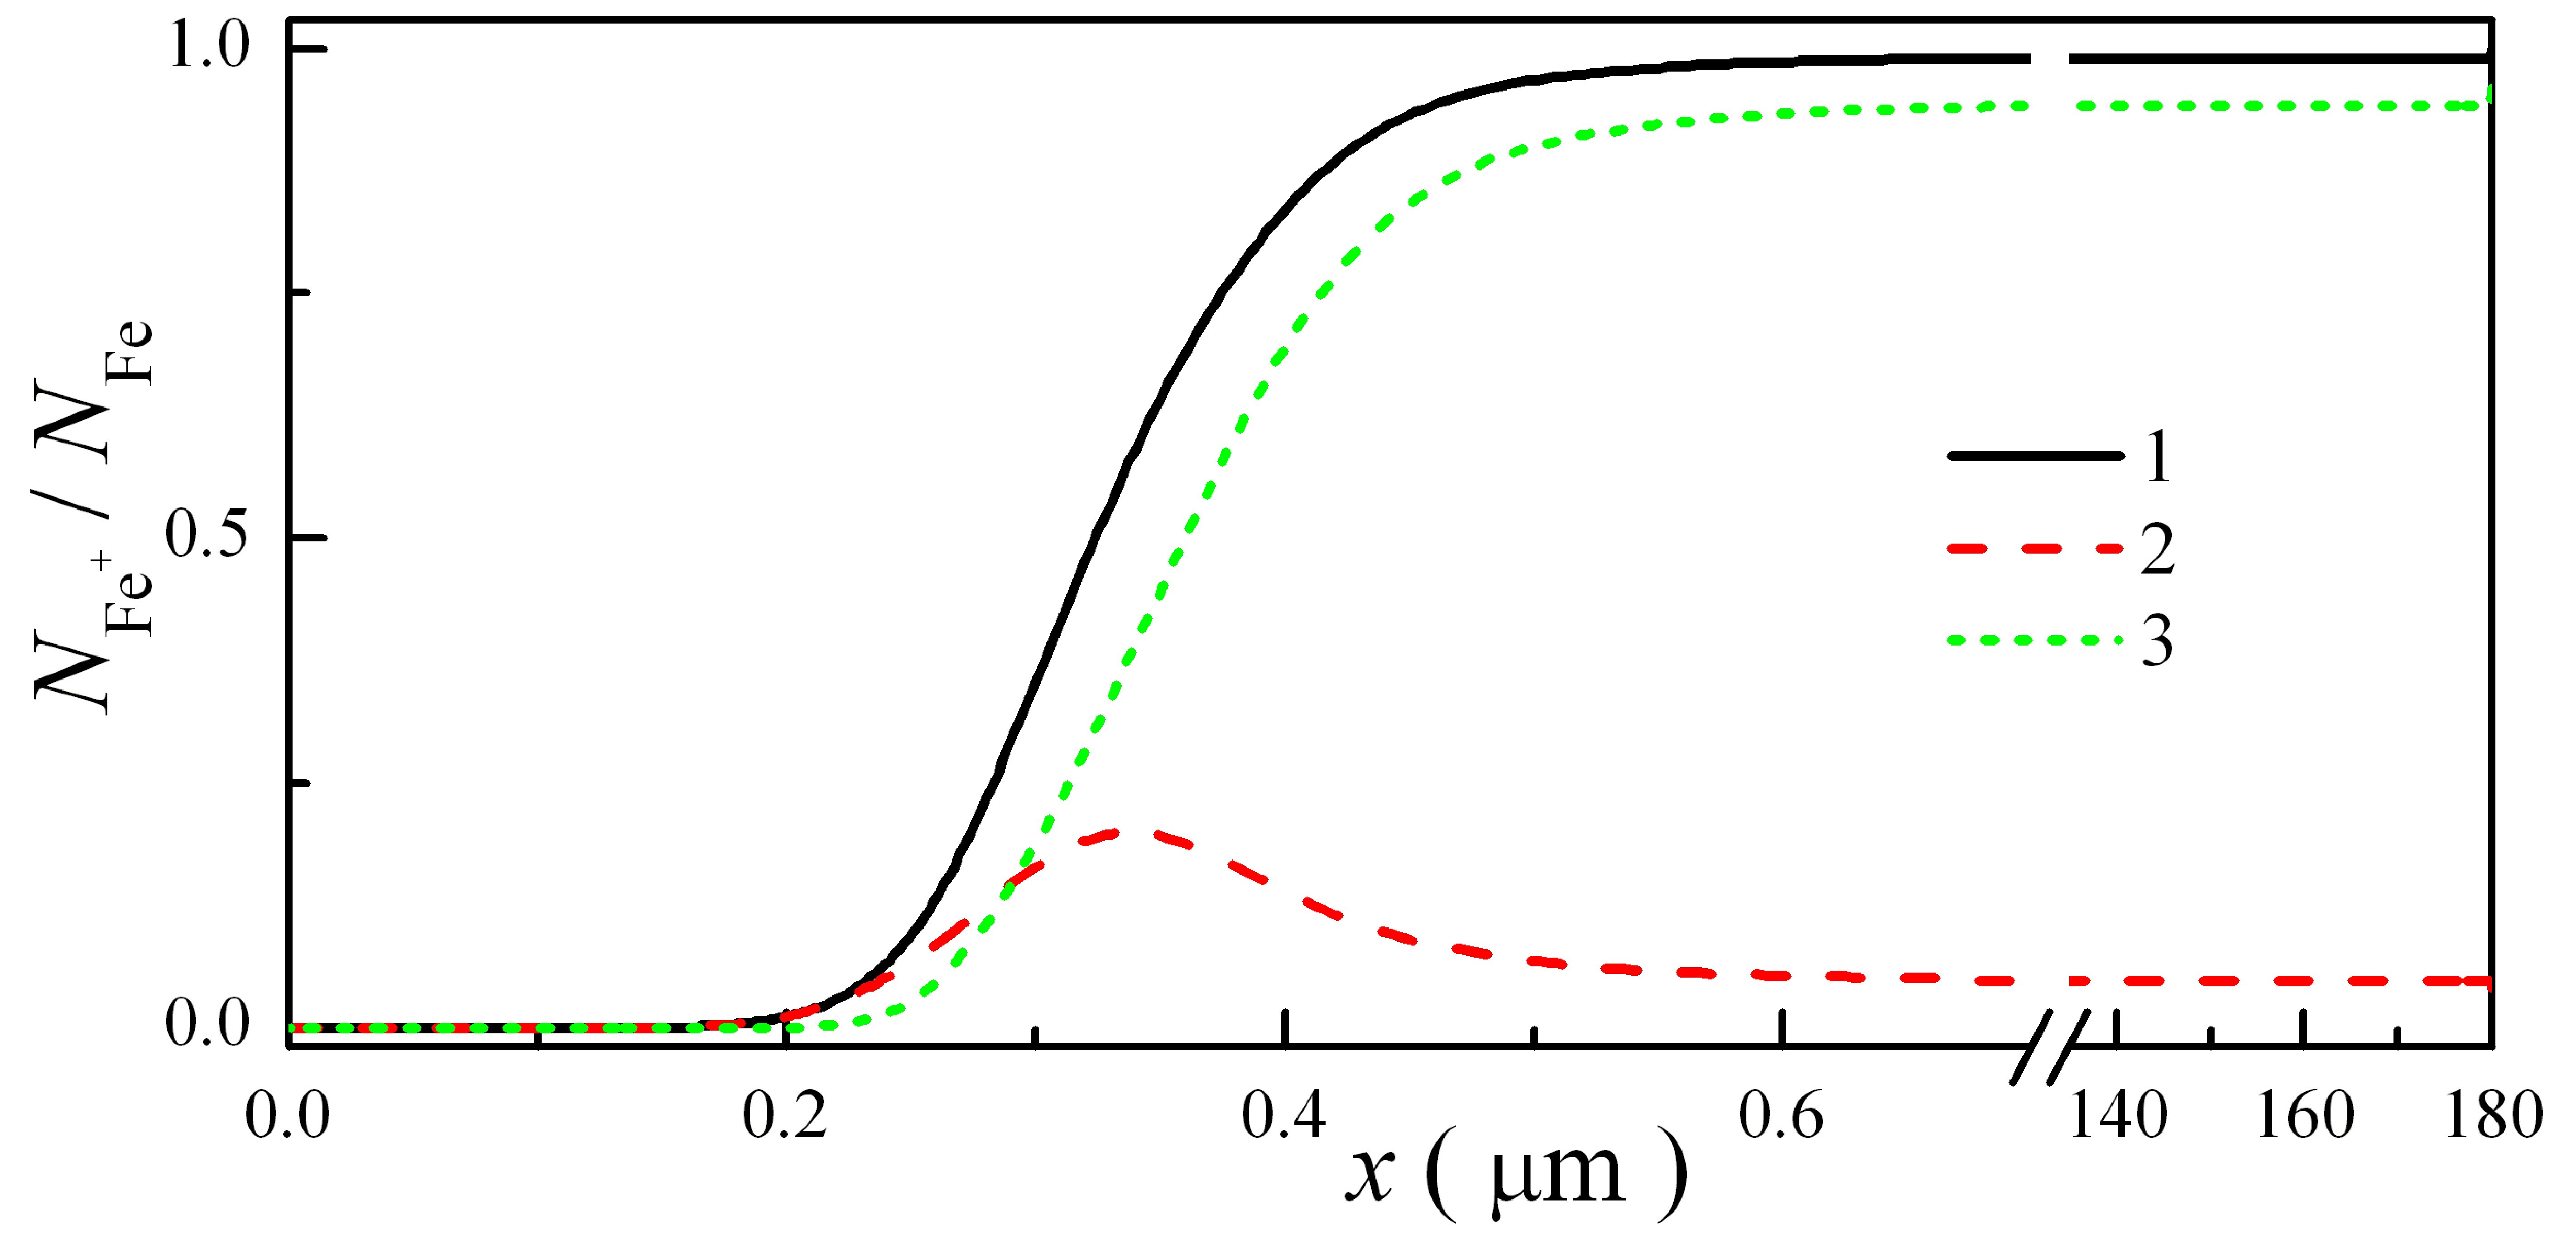
\includegraphics[width=7.5cm]{FigDelFei}
\caption{.
}
\label{FigDelFei}
\end{figure}

\newpage

\begin{center}
{\bfseries Моделювання фактору неідеальності в $n^+$--$p$--$p^+$--Si структурах}

О.Я. Оліх, O.В. Завгородній

\emph{Київський національний університет імені Тараса Шевченка}

\emph{Україна, 01601, місто Київ, вул. Володимирська, 64/13}

\emph{e-mail: olikh@univ.kiev.ua}

\end{center}

У цій роботі подано результати моделювання величини фактору неідеальності кремнієвих $n^+-p-p^+$ структур.
При цьому вважалося, що основні рекомбінаційні центри у базі структури пов'язані з домішковими атомами заліза.
Для моделювання вольт-амперних характеристик таких структур використовувався Solar Cells Capacitance Simulator (SCAPS). 
При цьому додатково враховувалися температурні залежності параметрів як матеріалу, так і дефектів.
При розрахунках вар'ювалися величини рівня легування ($10^{15}\div10^{17}$~см$^{-3}$ атомів бору) та товщини ($150\div240$~$\mu$м) бази,
температура ($290\div340$~K) та концентрації домішки заліза ($10^{10}\div10^{13}$~см$^{-3}$).
Окремо розглядалися випадки, коли всі атоми заліза знаходилися у міжвузольному положенні $\mathrm{Fe}_i$ та
коли переважна частина з них утворювала пари з легуючою домішкою $\mathrm{Fe}_i\mathrm{B}_s$.
Останній випадок відповідає стану рівноваги за відсутності освітлення і при цьому 
співвідношення між концентраціями  $\mathrm{Fe}_i$ та $\mathrm{Fe}_i\mathrm{B}_s$ визначалося положенням
рівня Фермі та температурою.
Визначення величини фактору неідеальності ($n$) відбувалося шляхом апроксимації (з використанням
метаеврістичного методу IJAVA) отриманих вольт-амперні характеристик.

Показано, що навіть за наявності $\mathrm{Fe}_i\mathrm{B}_s$ основну роль у формуванні величини $n$
відіграють процеси рекомбінації за участю рівнів, пов'язаних з $\mathrm{Fe}_i$.
Залежності $n$ від температури та рівня легування визначаються, насамперед,
заселеністю рівня $\mathrm{Fe}_i$.
У випадку, коли підсилюється відносний внесок процесів власної рекомбінації (високі 
температури та рівень легування, низькі концентрації домішки) відбувається зменшення фактору неідеальності.
На величину $n$, окрім концентрації дефектів, впливає також їх просторове розташування відносно $p-n$ переходу.
Зі збільшенням товщини бази структури (у випадку, коли вона перевищує довжину дифузії неосновних носіїв та
переважаючою є рекомбінація Шоклі-Ріда-Хола) відбувається незначне зменшення фактору неідеальності.
Показано, що можуть реалізуватися випадки, коли $n$ після розпаду $\mathrm{Fe}_i\mathrm{B}_s$ зменшується.
Запропоновано, що зміна фактору неідеальності поряд після розпаду $\mathrm{Fe}_i\mathrm{B}_s$ поряд з абсолютним значенням $n$  може бути використана
для оцінки концентрації домішок.


\textbf{Ключові слова:}
фактор неідеальності, кремній, $n^+$--$p$--$p^+$ структура, SCAPS, концентрація заліза


\end{document}
